\documentclass[lettersize,journal]{IEEEtran}

% =========================
% Packages
% =========================
% \usepackage[numbers,sort&compress]{natbib}
\usepackage{amsmath,amsfonts}
\usepackage{amssymb}
\usepackage{mathtools}
\usepackage{bm}

\usepackage{algorithm}
\usepackage{algorithmic}
\usepackage{booktabs}
\usepackage{threeparttable}
\usepackage{array}
\usepackage{multirow}
\usepackage{tabularx}
\usepackage{makecell}
\usepackage{graphicx}
\usepackage{stfloats}
\usepackage[table]{xcolor}
\usepackage{url}
\usepackage{cite}
\usepackage{textcomp}
\usepackage{verbatim}
\usepackage[final]{microtype}

\microtypesetup{protrusion=true,expansion=true}
\emergencystretch=2em
\hyphenpenalty=5000
\exhyphenpenalty=5000
\tolerance=1500
\hbadness=10000

\allowdisplaybreaks

% =========================
% Table / figure helpers
% =========================
\newcolumntype{Y}{>{\centering\arraybackslash}X}
\renewcommand\theadfont{\bfseries\footnotesize}
\newcommand{\best}[1]{\textbf{#1}}
\newcommand{\second}[1]{\underline{#1}}
\newcommand{\largest}[1]{\textbf{#1}}
\newif\ifincludeauthorbios
\includeauthorbiosfalse

\definecolor{TableHeader}{HTML}{E8EEF7}
\definecolor{RowProposed}{HTML}{E7F4EA}
\definecolor{RowBaseline}{HTML}{EAF1FB}
\definecolor{RowRisk}{HTML}{FFF3E1}
\definecolor{RowPhysical}{HTML}{F6EFE3}
\definecolor{RowScenario}{HTML}{EEF7F6}
\definecolor{RowBudget}{HTML}{F2F6E9}
\definecolor{RowNeutral}{HTML}{F4F4F4}
\definecolor{RowWeak}{HTML}{FBEAEA}

\renewcommand{\topfraction}{0.86}
\renewcommand{\dbltopfraction}{0.72}
\renewcommand{\textfraction}{0.14}
\renewcommand{\floatpagefraction}{0.76}
\renewcommand{\dblfloatpagefraction}{0.80}
\setcounter{topnumber}{2}
\setcounter{dbltopnumber}{1}
\setcounter{totalnumber}{3}
\setlength{\textfloatsep}{8pt plus 2pt minus 2pt}
\setlength{\dbltextfloatsep}{8pt plus 2pt minus 2pt}
\setlength{\floatsep}{8pt plus 2pt minus 2pt}
\setlength{\dblfloatsep}{8pt plus 2pt minus 2pt}
\hyphenation{op-tical net-works semi-conduc-tor IEEE-Xplore cyber-physical counterfactual malware resilience interdependent communication power-communication Safe-Guarded degradation-recovery}

\begin{document}

\title{Safe-Guarded Counterfactual Defense for Malware-Resilient Cyber--Physical Power Systems}

\author{
Weihao~Cheng,
Haicheng~Tu,~\IEEEmembership{Member,~IEEE},
Youjia~Ling,
Yongxiang~Xia,~\IEEEmembership{Senior~Member,~IEEE},
and~Xi~Chen,~\IEEEmembership{Senior~Member,~IEEE}%

\thanks{
Weihao Cheng, Haicheng Tu, and Yongxiang Xia are with the School of Communication Engineering, Hangzhou Dianzi University, Hangzhou 310018, China.\\
Youjia Ling is with the School of Accounting, Hangzhou Dianzi University, Hangzhou 310018, China.\\
Xi Chen is with the Department of Artificial Intelligence, China Electric Power Research Institute, Beijing 100192, China.\\
Corresponding author: Haicheng Tu.\\
E-mail: weihao\_cheng@hdu.edu.cn; tuhc@hdu.edu.cn; 24140511@hdu.edu.cn; xiayx@hdu.edu.cn; xc@ieee.org.
}
}

\markboth{IEEE Transactions on Network Science and Engineering}%
{Cheng \MakeLowercase{\textit{et al.}}: Safe-Guarded Counterfactual Defense for Malware-Resilient CPPSs}

\maketitle

\begin{abstract}
Malware propagation in cyber--physical power systems (CPPSs) can turn local communication-layer compromise into physical affected-service degradation, measured here by the physics-informed percentage of affected service, and a subsequent recovery burden. Existing protection rules usually rank nodes once by topology or physical importance, so they cannot respond to changing infection states, coupling patterns, attack timing, and defense budgets. This paper proposes a dynamic risk-aware counterfactual model predictive defense framework, termed DRAD-CF-MPC, for malware-resilient CPPSs. DRAD-CF-MPC evaluates node-level cyber--physical risk from communication centrality, coupled physical consequence, infection exposure, and attacker-information uncertainty, and then compares interpretable candidate policies through same-state counterfactual rollouts. A Safe-Guard rule accepts policy switching only when the predicted improvement over communication-degree protection (CDP), the strongest fixed baseline, is sufficiently reliable. Experiments on an IEEE 118-bus system coupled with a scale-free communication network show that DRAD-CF-MPC reduces the mean attacker expected payoff by 63.2\% compared with no protection and achieves a 6.20\% mean scenario-level gain over CDP. The results show that conservative counterfactual adaptation improves CPPS resilience without abandoning interpretable engineering rules.
\end{abstract}

\begin{IEEEkeywords}
Cyber--physical power systems, malware propagation, network resilience, adaptive defense, model predictive control.
\end{IEEEkeywords}



\section{Introduction}

\IEEEPARstart{C}{yber}--physical power systems (CPPSs) increasingly rely on communication networks for monitoring, protection, and control. This coupling improves situational awareness, yet it also creates a path by which a cyber disturbance can become physical service degradation. A malware infection that is initially confined to communication devices may spread through the cyber layer, compromise nodes coupled to power buses, and eventually increase affected service. This cross-layer risk is consistent with the broader observation that interdependent infrastructures may propagate failures across functional layers rather than absorb them locally \cite{rinaldi2001interdependencies}. It is also consistent with network-science results showing that dependency links can amplify cascading failures and create abrupt degradation \cite{buldyrev2010catastrophic}.

For CPPSs, the challenge is not only to model this cross-layer propagation, but also to make closed-loop defense decisions while the cyber state is evolving. Existing malware-resilience studies have made important progress by describing malware incubation, attacker information, and coupling patterns \cite{xu2020analysis}, and network-science studies have further addressed attacked-area detection and post-attack information recovery in power grids \cite{soltan2019react}. More recent studies further analyze robustness under attack--defense confrontation and malware incubation settings \cite{xu2023resilience,zhang2025robustness}. A common limitation remains: the defender is usually represented by a fixed node-ranking rule, such as protecting high-degree communication nodes, high-degree power buses, high-capacity buses, or randomly selected nodes. Such rules are interpretable, but they do not ask whether the same rule remains appropriate after the infection distribution, coupling pattern, budget, and attack timing change.

This paper starts from the observation that malware defense in CPPSs has two competing requirements. On the one hand, the defender should be adaptive: when the current infection state or cyber--physical coupling reveals a better allocation, the policy should move beyond a static ranking. On the other hand, the defender should be conservative: in critical infrastructures, an adaptive policy should not abandon a strong and interpretable baseline unless the expected gain is reliable. A method that only pursues adaptivity may switch for noisy gains, while a method that only preserves a fixed baseline can miss scenario-dependent opportunities.

The same tension appears in evaluation. A defense strategy that only reduces peak damage may still leave a large recovery burden, while a strategy that modestly changes the peak can substantially improve the subsequent restoration trajectory. Therefore, the defense objective should connect malware diffusion, affected power buses, the physics-informed percentage of affected service (PAS), and post-attack recovery in one assessment chain, instead of treating cyber containment and physical resilience as separate problems \cite{li2024review,zhao2024improving}.

The resulting gap is a network-science decision gap rather than only a metric-design gap. The defender needs a mechanism that can compare several interpretable protection principles under the same observed network state, account for cyber-to-physical consequences, and avoid unstable switching when a strong baseline remains competitive. This perspective motivates a conservative form of adaptation: policy changes should be allowed, but only after same-state counterfactual evidence indicates that the change is likely to reduce affected service and recovery burden.

The central novelty of this work is therefore not another isolated centrality score. Instead, the goal is to turn a set of interpretable network-defense rules into a closed-loop decision process. This distinction is important for CPPS defense. A communication hub may be the right node to protect when malware diffusion dominates, a physically important coupled bus may matter more when cyber compromise is already close to high-impact loads, and a hybrid rule may be preferable when coupling structure changes the cyber-to-physical pathway. A fixed rule cannot express this conditional logic, while a black-box controller would be difficult to justify for critical infrastructure protection. DRAD-CF-MPC is designed to occupy the middle ground: it keeps the candidate actions interpretable, but evaluates them dynamically under the same observed state.

Another novelty is the Safe-Guarded use of counterfactual lookahead. In a stochastic malware process, a candidate policy may appear better because of rollout noise or because it overfits one scenario. Directly switching to such a policy can make an adaptive defense less reliable than a strong static baseline. The proposed Safe-Guard rule treats communication-degree protection (CDP) as an engineering anchor and accepts a switch only when the predicted multi-metric improvement exceeds a switching margin and the paired affected-service improvement remains positive under common random seeds. Thus, the framework is adaptive by design, but conservative in execution. This focus on conservative counterfactual adaptation is the organizing principle of the paper.

To address these issues, this paper proposes a Dynamic Risk-Aware Defense with Counterfactual Model Predictive Control, abbreviated as DRAD-CF-MPC\footnote{The source code and experimental configurations are publicly available at \url{https://github.com/VhoCheng/DRAD-CF-MPC}.}. The framework evaluates cyber--physical node risk from communication centrality, coupled physical consequence, infection exposure, and attacker-information uncertainty. It then compares interpretable candidate policies from the same observed state through counterfactual rollouts. A Safe-Guard rule accepts policy switching only when the candidate policy provides a reliable gain over a strong communication-degree baseline. The contributions are summarized as follows.
\begin{enumerate}
    \item \textbf{Closed-loop CPPS malware defense.} Malware defense is reformulated from a fixed ranking task into a state-dependent decision problem driven by infection state, coupling structure, defense budget, and physical consequence. This makes the defense action responsive to the current cyber--physical condition rather than tied to one global notion of node importance.
    \item \textbf{Counterfactual MPC with Safe-Guarded switching.} Candidate policies are evaluated by same-state rollouts with common random seeds, and adaptive switching is accepted only when the predicted improvement over a strong baseline is sufficiently reliable. The Safe-Guard rule is used to preserve the robustness of CDP while still exploiting scenario-dependent gains.
    \item \textbf{Unified degradation--recovery defense objective.} By incorporating malware diffusion, PAS, and post-attack restoration trajectory into a single counterfactual evaluation objective (Eq.~\eqref{eq:counterfactual_objective}), DRAD-CF-MPC makes defense decisions that jointly suppress peak affected service and reduce recovery burden---a coupling absent from prior fixed-ranking defenses that optimize node importance independently of restoration cost.
\end{enumerate}

The remainder of this paper is organized as follows. Section~\ref{sec:related_work} reviews related work and identifies the research gap. Section~\ref{sec:system_model} formulates the CPPS model and evaluation metrics. Section~\ref{sec:method} presents DRAD-CF-MPC. Section~\ref{sec:experimental_setup} describes the experimental protocol. Section~\ref{sec:results} reports simulation results and discussion. Section~\ref{sec:conclusion} concludes the paper.

\section{Related Work}
\label{sec:related_work}

The starting point of this study is the networked nature of CPPS failures. Interdependent-infrastructure research shows that failures in one layer can change the operating condition of another layer \cite{ouyang2014review}. Network-of-networks studies further show that dependency structure may turn local disturbances into system-level fragility \cite{vespignani2010complex,gao2012networks}. Multilayer-network theory explains why coupling can alter spreading thresholds, vulnerability patterns, and robustness \cite{kivela2014multilayer,boccaletti2014structure}. In this view, malware propagation is not merely a cyber-security event. Once infected communication nodes are coupled to power buses, the cyber diffusion process becomes a driver of physical service degradation. Epidemic spreading on multilayer networks and classical complex-network results provide the analytical background for such cross-layer propagation \cite{salehi2015spreading,barabasi1999emergence}. They also explain why hubs and dependency interfaces often dominate diffusion and robustness \cite{albert2000error,newman2003structure}. Cascading-attack models and blackout studies reach the same conclusion from different directions: rare severe events are shaped by interacting network pathways rather than by isolated component failures \cite{motter2002cascade,dobson2007complex,hines2009large}.

Smart-grid security studies then clarify how cyber compromise can materialize as physical risk. Broad CPPS and smart-grid security surveys identify the power grid as a coupled attack surface in which sensing, communication, control, and physical operation cannot be separated \cite{sridhar2012cyber,he2016cyberphysical}. General cyber--physical security surveys reach the same conclusion across infrastructure domains \cite{humayed2017cyber}. False-data injection and cyber--physical attack models demonstrate that cyber manipulation may affect state estimation, dispatch, and physical operating margins \cite{ten2010cybersecurity,mo2012cyber}. Load-redistribution and strategic-protection studies make this physical consequence explicit by linking cyber manipulation to line stress, load stress, and operating damage \cite{yuan2011modeling,kim2011strategic,liu2009false}. Secure-control and moving-target-defense studies further suggest that cyber defense should be treated as a survivability and adaptation problem \cite{cardenas2008secure,cho2020proactive,griffioen2021moving}. Recent botnet-oriented CPPS analysis reinforces the same point under dynamic malware-like attack processes \cite{zhao2024iotbotnet}. These studies motivate adaptive protection, but they do not directly answer which communication nodes should be protected when malware diffusion, coupling structure, physical consequence, and restoration burden evolve together.

CPPS malware studies move closest to the decision problem considered here. Existing work has modeled malware-induced attacks, incubation periods, detection probability, and attack information on coupled power--communication networks \cite{xu2020analysis}, while graph-theoretic studies have developed detection and recovery mechanisms against cyber attacks that jointly affect grid data and physical operation \cite{soltan2019react}. Later studies extend the analysis to renewable CPPS resilience and attack--defense confrontation \cite{xu2023resilience,zhang2025robustness}. The key insight from this line of work is that a cyber infection should be evaluated through its physical consequence. The remaining gap is the defense mechanism: most defenses are still evaluated as fixed ranking rules. They can identify important nodes, but they do not provide a closed-loop answer to when the defender should keep a strong baseline and when it should switch to another interpretable policy.

Resilience studies add the final piece of the problem. Power-system resilience is not fully described by the attack peak; the time and efficiency of recovery also matter \cite{mahzarnia2020review,younesi2022trends}. Cyber-physical resilience definitions emphasize the ability to withstand, adapt to, and recover from disruptive cyber--physical events \cite{arghandeh2016definition}. Recent CPPS resilience studies also stress that mitigation must reflect the dual cyber and physical nature of the infrastructure \cite{ding2024dual}. Resilience metrics based on affected service and restoration trajectories have been widely used to evaluate disruptive events in power systems \cite{panteli2015influence,panteli2017metrics}. For malware-resilient CPPS defense, this means that node protection should be judged by the complete chain from cyber diffusion to physical degradation and recovery. DRAD-CF-MPC is designed for this gap: it keeps the interpretability of ranking-based policies, adds counterfactual closed-loop evaluation, and uses Safe-Guarded fallback to avoid unreliable adaptation.

\section{System model and problem formulation}
\label{sec:system_model}

This section defines only the quantities used in the simulation pipeline: the coupled power--communication topology, the malware propagation state, the mapping from infected communication nodes to affected power buses, the physical-consequence proxy, the defense budget, and the evaluation metrics. The model follows the implemented state-to-consequence chain: malware evolves in the cyber layer, compromised communication nodes affect coupled power buses, affected buses create PAS, and the remaining affected service determines the restoration burden.

\subsection{Interdependent power--communication network}
\label{subsec:cpps_network}

A cyber-physical power system (CPPS) is represented by a physical power network $\mathcal{G}^{p}=(\mathcal{V}^{p},\mathcal{E}^{p})$ and a communication network $\mathcal{G}^{c}=(\mathcal{V}^{c},\mathcal{E}^{c})$, where $N_p=|\mathcal{V}^{p}|$ and $N_c=|\mathcal{V}^{c}|$. In the experiments, $\mathcal{G}^{p}$ is the IEEE 118-bus system and $\mathcal{G}^{c}$ is a 118-node Barabasi--Albert scale-free network. The cyber--physical coupling is described by a binary matrix
\begin{equation}
    \mathbf{M}=[m_{uv}]\in\{0,1\}^{N_c\times N_p},
    \label{eq:coupling_matrix}
\end{equation}
where $m_{uv}=1$ indicates that communication node $u$ is coupled to power bus $v$. The set of buses coupled to node $u$ is
\begin{equation}
    \mathcal{C}(u)=\{v\in\mathcal{V}^{p}\mid m_{uv}=1\}.
    \label{eq:coupled_bus_set}
\end{equation}
If a communication node is coupled to multiple buses, its physical-side feature is aggregated as the mean of the corresponding bus features, e.g., $\bar{z}_{\mathcal{C}(u)}^{p}=|\mathcal{C}(u)|^{-1}\sum_{v\in\mathcal{C}(u)}\bar{z}_{v}^{p}$. The experiments use degree-correlated, degree-disassortative, and random coupling patterns to test whether the defense method is robust to different interdependency structures.

\subsection{Malware propagation and protection}
\label{subsec:malware_model}

Each communication node $u$ has a discrete state $x_u(t)\in\{S,E,I,D,P\}$, where $S$, $E$, $I$, $D$, and $P$ denote susceptible, exposed, infectious, detected/disabled, and protected, respectively. Fig.~\ref{fig:malware_state_transition} illustrates the corresponding state-transition and protection mechanism. For a susceptible and unprotected node, the implemented infection probability is

\begin{figure}[!t]
    \centering
    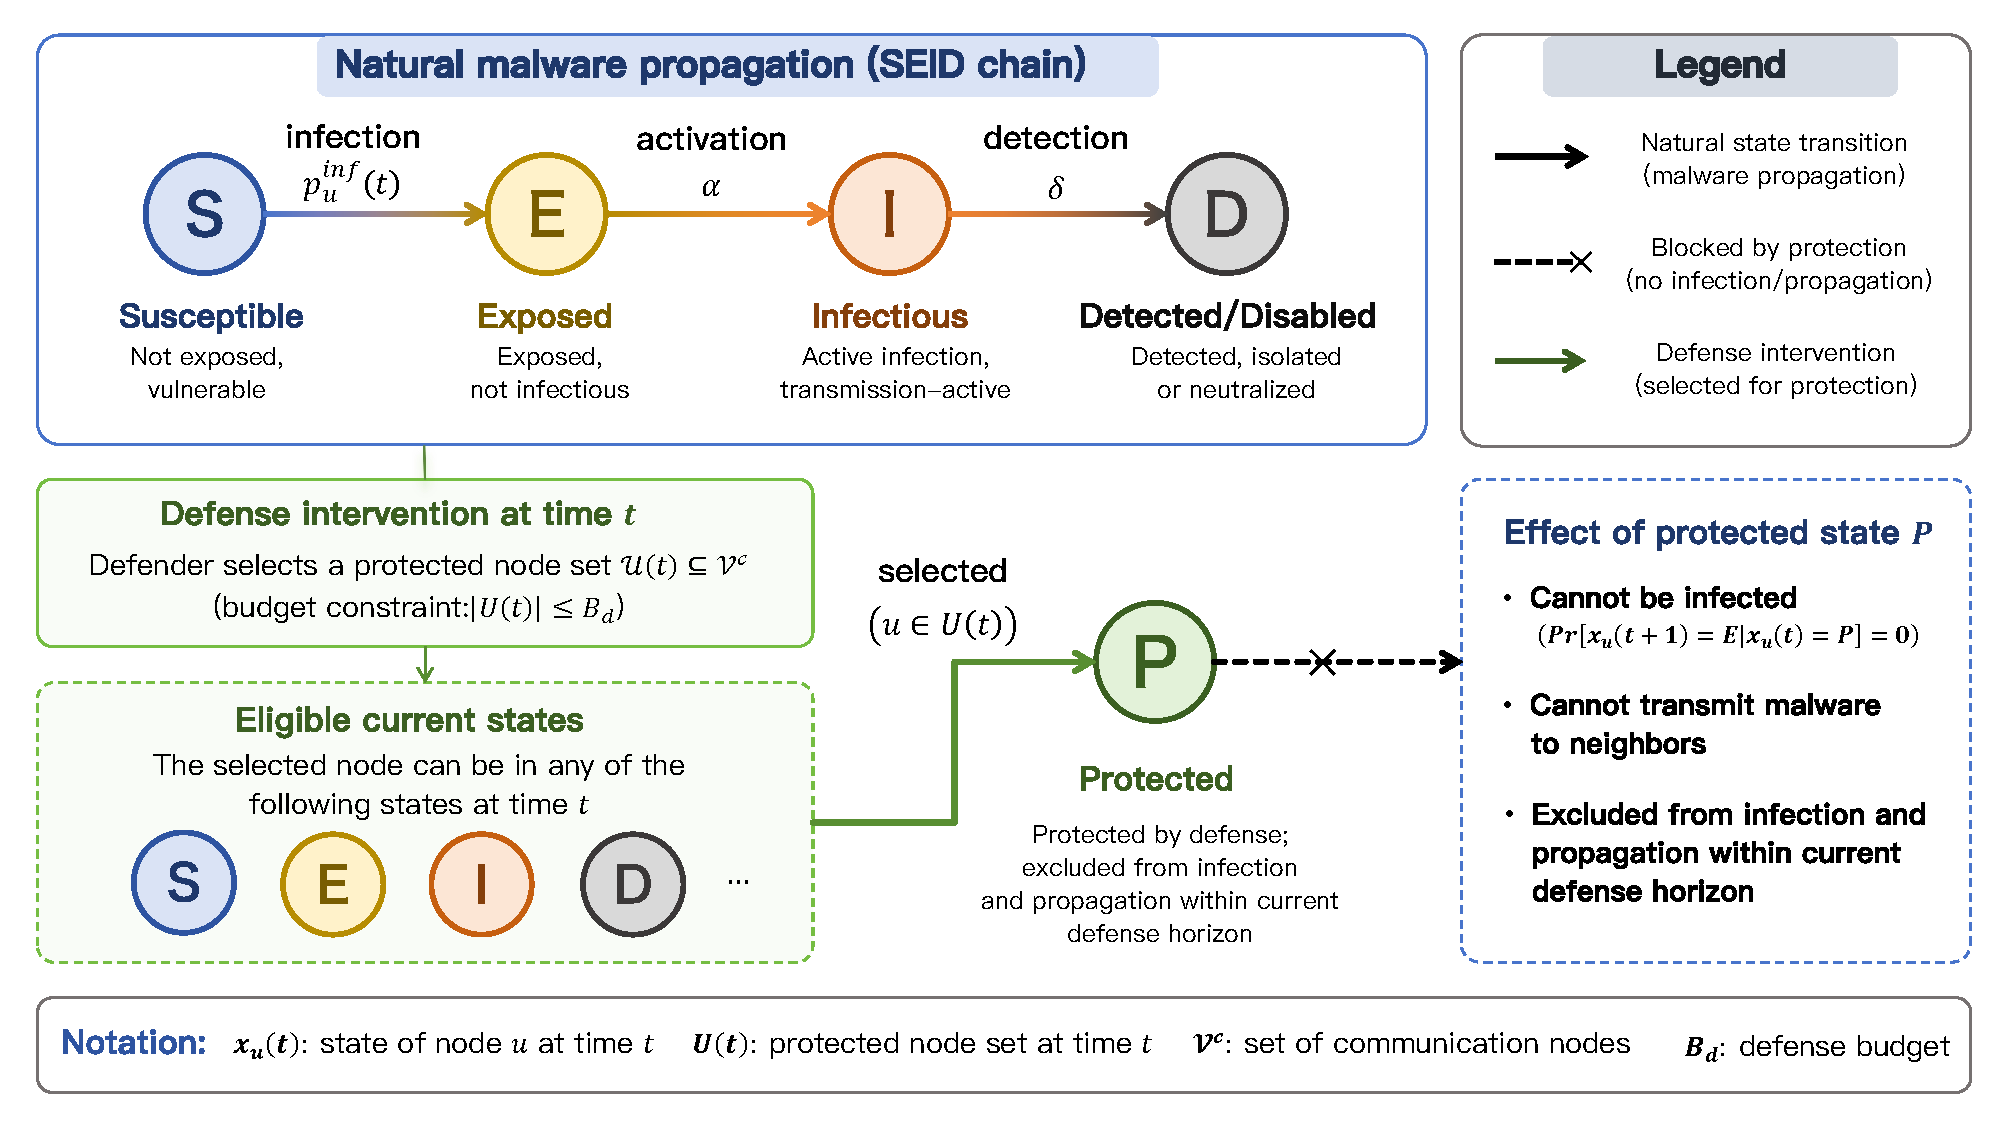
\includegraphics[width=\columnwidth]{figures/Figure_supply.pdf}
    \caption{State-transition diagram of malware propagation and protection.}
    \label{fig:malware_state_transition}
\end{figure}

\begin{equation}
    p_u^{\mathrm{inf}}(t)
    =
    1-
    \prod_{j\in\mathcal{N}_{c}(u)}
    \left(1-\beta\,\mathbb{I}[x_j(t)=I]\right),
    \label{eq:infection_prob}
\end{equation}
where $\mathcal{N}_{c}(u)$ is the cyber-neighbor set, $\beta$ is the infection rate, and $\mathbb{I}[\cdot]$ is the indicator function. An exposed node becomes infectious with probability $\alpha$, and an infectious node is detected with probability $\delta$:
\begin{equation}
\begin{aligned}
    \Pr[x_u(t+1)=I\mid x_u(t)=E]&=\alpha,\\
    \Pr[x_u(t+1)=D\mid x_u(t)=I]&=\delta .
\end{aligned}
    \label{eq:activation_detection}
\end{equation}
The detected/disabled state is absorbing in the malware horizon, i.e., a detected node is treated as neutralized and does not return to the susceptible state in the reported simulations. A protected node is also unavailable for infection and transmission during the current defense horizon. The defender selects a protected node set $\mathcal{U}(t)\subseteq\mathcal{V}^{c}$ under the budget
\begin{equation}
    |\mathcal{U}(t)|\leq B_d .
    \label{eq:defense_budget}
\end{equation}

\subsection{Cyber-to-physical consequence model}
\label{subsec:degradation_model}

Let $t_{\mathrm{on}}$ denote the physical attack activation time, and let
\[
\widetilde{\mathcal{A}}^{p}(t)=
\{v\in\mathcal{V}^{p}\mid \exists u\in\mathcal{V}^{c},
m_{uv}=1,\,x_u(t)\in\{I,D\}\}.
\]
The state $P$ is mutually exclusive with $I$ and $D$; after the defense update, a protected node has $x_u(t)=P$ and is therefore excluded from $\widetilde{\mathcal{A}}^{p}(t)$. Infectious or disabled communication nodes affect their coupled buses only after this activation time:
\begin{equation}
    \mathcal{A}^{p}(t)
    =
    \begin{cases}
    \widetilde{\mathcal{A}}^{p}(t), & t\geq t_{\mathrm{on}},\\
    \emptyset, & t<t_{\mathrm{on}} .
    \end{cases}
    \label{eq:affected_buses}
\end{equation}
The number of affected buses is $B(t)=|\mathcal{A}^{p}(t)|$.

To match the simulation implementation, the physical consequence is quantified by a physics-informed bus impact score. Let $\widetilde{P}^{L}_{v}$, $\widetilde{C}_{v}$, $\widetilde{k}^{p}_{v}$, and $\widetilde{b}^{p}_{v}$ denote the normalized load demand, capacity proxy, power degree, and power betweenness of bus $v$, respectively. For any raw bus feature $z_v$, the normalized value is computed by min--max scaling,
\begin{equation}
    \widetilde{z}_v
    =
    \frac{z_v-z_{\min}}{z_{\max}-z_{\min}+\varepsilon_0},
    \label{eq:minmax_normalization}
\end{equation}
where $z_{\min}=\min_{\ell\in\mathcal{V}^{p}}z_\ell$, $z_{\max}=\max_{\ell\in\mathcal{V}^{p}}z_\ell$, and $\varepsilon_0$ is the numerical stabilizer used in all denominator normalizations. The raw capacity proxy $C_v$ is the bus-level physical service-capacity feature used by the CP baseline; it is constructed once from the power-network data and then normalized by Eq.~\eqref{eq:minmax_normalization}. The bus impact score is
\begin{equation}
\begin{aligned}
    \phi_v
    =
    &\omega_L\widetilde{P}^{L}_{v}
    +\omega_C\widetilde{C}_{v}\\
    &+\omega_k\widetilde{k}^{p}_{v}
    +\omega_b\widetilde{b}^{p}_{v},
\end{aligned}
    \label{eq:bus_impact_score}
\end{equation}
where $\omega_L,\omega_C,\omega_k,\omega_b\geq0$ and $\omega_L+\omega_C+\omega_k+\omega_b=1$. The experiments use $(\omega_L,\omega_C,\omega_k,\omega_b)=(0.35,0.25,0.20,0.20)$, which assigns the largest weight to load demand as the most direct indicator of affected service to end users, a secondary weight to capacity as the principal supply-side constraint, and equal residual weights to power degree and betweenness as structural discrimination features among buses of comparable load and capacity. The weight vector is fixed before evaluation, kept identical for all strategies and scenarios, and not tuned from the reported results. Because the experiments use this service-impact proxy rather than solving an optimal power flow problem at every malware step, the physical consequence is reported as the physics-informed percentage of affected service (PAS):
\begin{equation}
    \mathrm{PAS}(t)
    =
    \frac{\sum_{v\in\mathcal{A}^{p}(t)}\phi_v}
    {\sum_{v\in\mathcal{V}^{p}}\phi_v+\varepsilon_0},
    \label{eq:pas}
\end{equation}
where the same $\varepsilon_0$ prevents division by zero and has no modeling role. This proxy preserves the implemented cyber-to-physical logic: malware determines infected communication nodes, coupling maps them to affected buses, and bus impact scores quantify affected service. Peak PAS values reported in the dynamic-evolution analysis are obtained directly from the trajectory of $\mathrm{PAS}(t)$.

\subsection{Evaluation metrics and defense objective}
\label{subsec:metrics}

For a defense policy $\pi$, stochastic malware simulations produce the attack-success probability $P_s^\pi(t)$ and the mean physical affected-service ratio $\overline{\mathrm{PAS}}_\pi(t)$. The expected attacker payoff used in the experiments is
\begin{equation}
    \mathrm{EP}_{\pi}(t)
    =
    \overline{\mathrm{PAS}}_\pi(t)\,P_s^\pi(t).
    \label{eq:expected_payoff}
\end{equation}
This quantity is not a monetary payoff. It is a composite attack-impact score: $P_s^\pi(t)$ measures whether the malware attack succeeds, while $\overline{\mathrm{PAS}}_\pi(t)$ measures the affected-service severity conditional on the simulated scenario ensemble. Their product therefore captures the joint probability--severity effect of a successful cyber-to-physical attack. The worst attack timing is summarized by
\begin{equation}
    \mathrm{EP}_{\max}^{\pi}
    =
    \max_{t\in\{0,\ldots,T\}}\mathrm{EP}_{\pi}(t),
    \label{eq:epmax}
\end{equation}
where $T$ is the malware simulation horizon.

Restoration-oriented performance is reported by restoration time (RT), resilience index (RI), and restoration efficiency (RE). These indicators are computed from the simulated affected-service ratio and defense budget in the experimental pipeline, and they are used only as evaluation outputs rather than as additional decision variables. RE is therefore an auxiliary recovery-efficiency indicator, not a separate control objective. Lower $\mathrm{EP}_{\max}$, PAS, and RT indicate stronger defense, while higher RI and RE indicate better retained service and recovery efficiency.

The observed state is
\begin{equation}
    s(t)=\big(\mathbf{x}(t),\mathbf{M},r_a,B_d,t_{\mathrm{on}}\big),
    \label{eq:observed_state}
\end{equation}
where $\mathbf{x}(t)=\{x_u(t)\}_{u\in\mathcal{V}^{c}}$ is the malware-state vector, $\mathbf{M}$ is the cyber--physical coupling matrix, $r_a$ is the attacker-information ratio, $B_d$ is the defense budget, and $t_{\mathrm{on}}$ is the physical attack activation time. The defense problem is therefore to choose a feasible policy $\pi$ that maps the observed cyber--physical state to a protected node set,
\begin{equation}
    \pi:s(t)\mapsto\mathcal{U}(t),\qquad |\mathcal{U}(t)|\leq B_d,
    \label{eq:policy_mapping}
\end{equation}
so as to reduce $\mathrm{EP}_{\max}$ and PAS while improving restoration-oriented metrics. Because the malware process is stochastic and the best defense ranking changes with infection state, coupling pattern, budget, and attack timing, the next section develops a dynamic risk-aware counterfactual MPC defense that approximates this objective through finite-horizon lookahead and Safe-Guarded policy switching.

\section{Dynamic Risk-Aware Counterfactual MPC Defense}
\label{sec:method}

This section presents DRAD-CF-MPC. The method is built around a simple principle: a CPPS defender should not choose a protection rule only because it is globally important; it should choose the rule that is expected to work best for the current infection state, coupling pattern, defense budget, and attack timing. At the same time, the method should not switch away from a strong baseline unless the counterfactual evidence is reliable. DRAD-CF-MPC therefore combines dynamic risk scoring, a finite library of interpretable defense policies, same-state counterfactual rollouts, and a CDP-anchored Safe-Guard rule.

\begin{figure*}[!tbp]
    \centering
    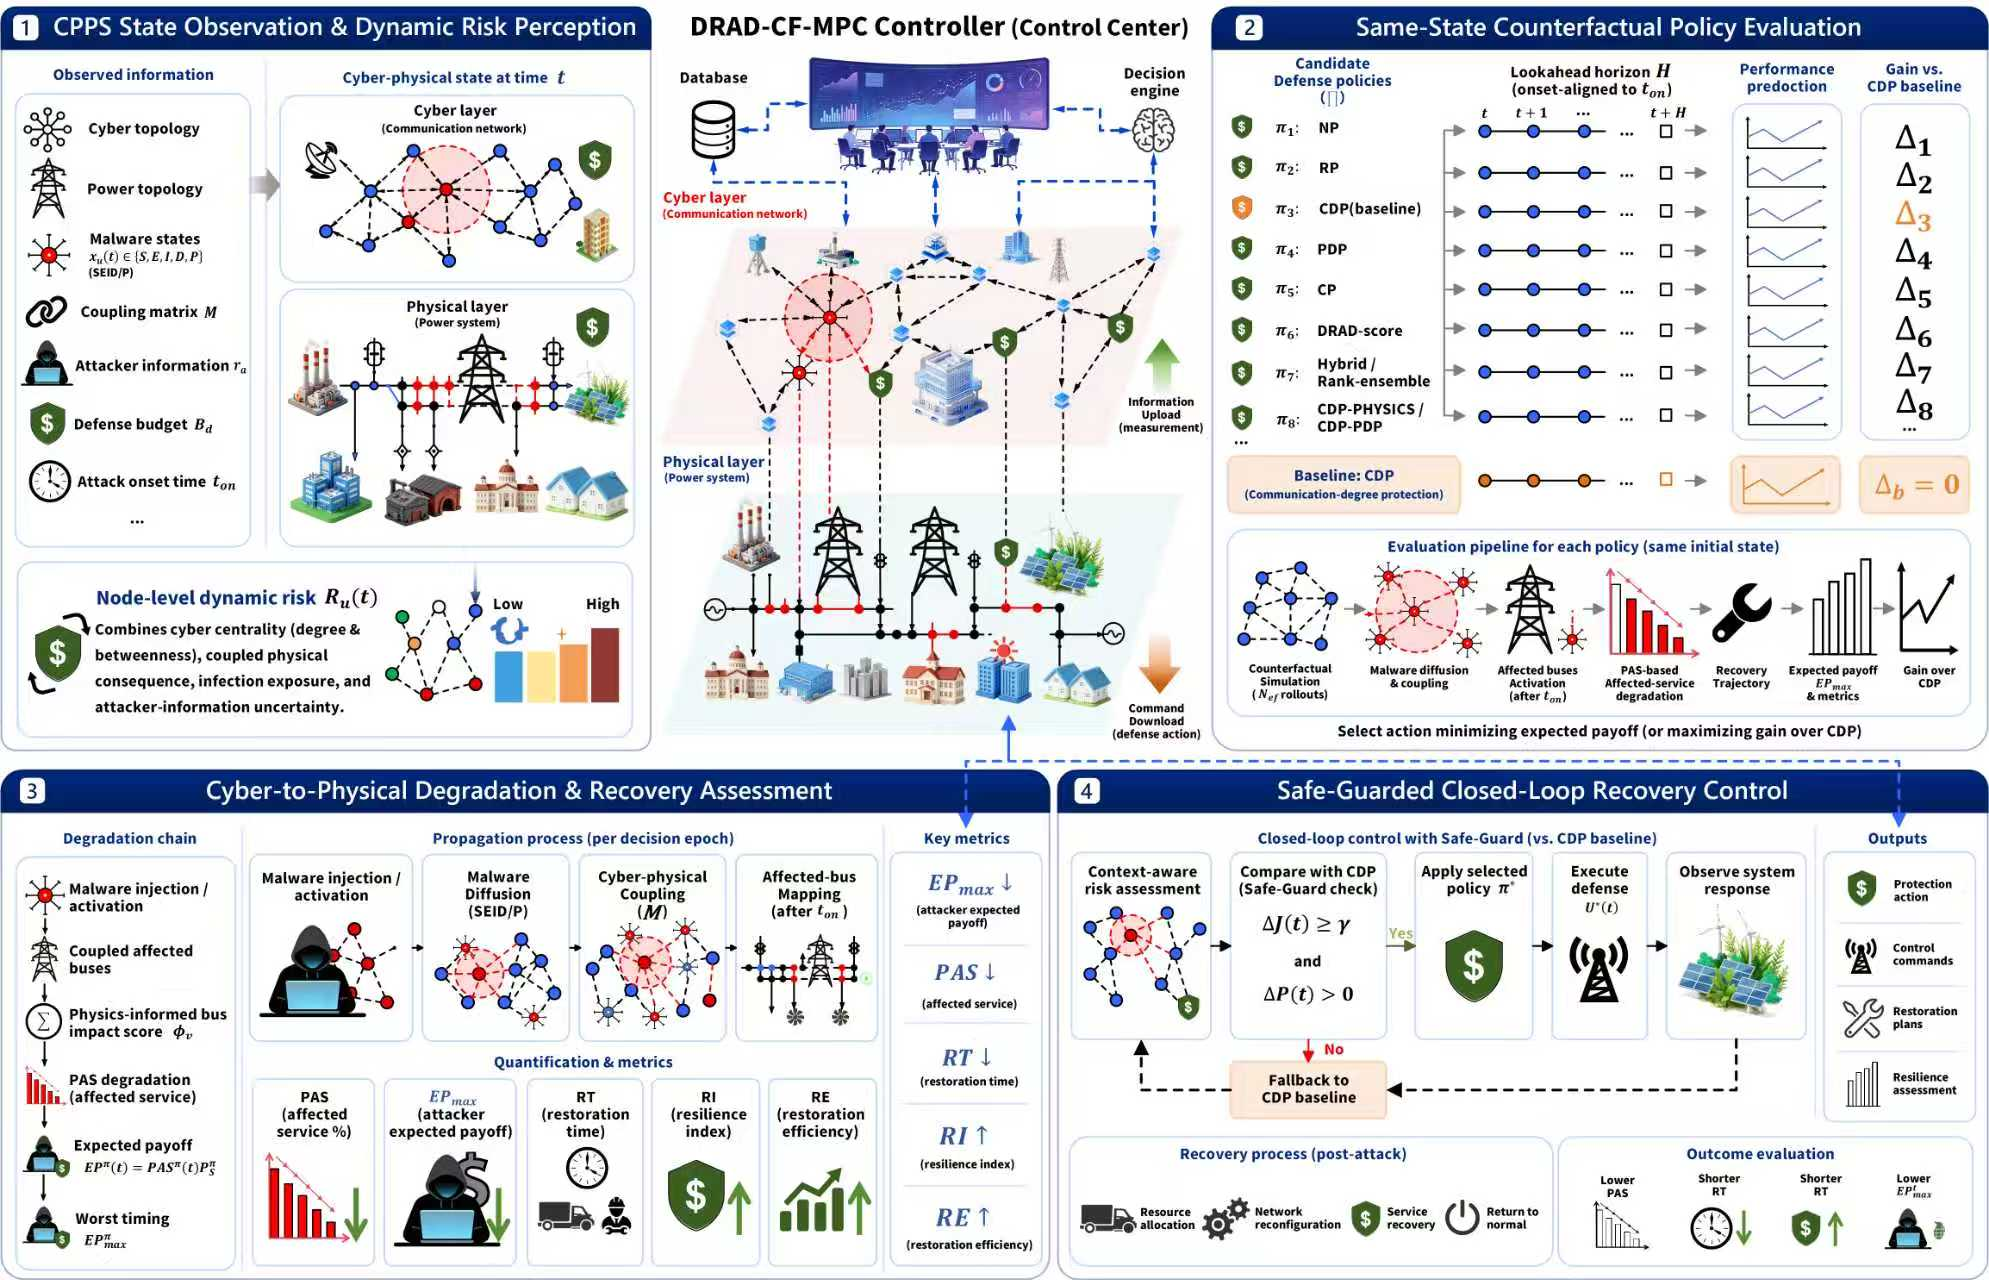
\includegraphics[width=0.98\textwidth]{figures/Figure1_overall_framework-revised.png}
    \caption{Overview of the proposed Safe-Guarded counterfactual network defense framework.}
    \label{fig:framework}
\end{figure*}

\subsection{Closed-loop decision workflow}
\label{subsec:method_overview}

Fig.~\ref{fig:framework} illustrates the workflow. At a decision epoch, the defender observes the malware state, exposed and infectious nodes, coupling pattern, attacker-information level, attack onset time, and defense budget. DRAD-CF-MPC then performs four steps. First, it constructs dynamic node scores from cyber topology, coupled physical consequence, local infection pressure, and information exposure. Second, it generates candidate node sets using interpretable policies. Third, it evaluates these candidates with common-random-number counterfactual rollouts initialized from the same observed state. Fourth, it executes the best candidate only if it passes the Safe-Guard test against the CDP baseline.

The method follows the receding-horizon idea of model predictive control \cite{camacho2013model,rawlings2017model}, but it does not solve an unconstrained high-dimensional control problem. Its search space is intentionally restricted to interpretable candidate policies so that each selected action can be explained as hub protection, physical-impact protection, hybrid protection, risk-aware ranking, or conservative fallback.

\subsection{Dynamic cyber--physical risk assessment}
\label{subsec:dynamic_risk}

For each communication node $u$, the dynamic risk score uses exactly the feature groups implemented in the simulation code. Let $\bar{k}_u^{c}$ and $\bar{b}_u^{c}$ denote normalized communication degree and betweenness. Let $\bar{k}_{\mathcal{C}(u)}^{p}$ and $\bar{c}_{\mathcal{C}(u)}^{p}$ denote the coupled physical degree and capacity-proxy features aggregated from the buses in $\mathcal{C}(u)$:
\begin{equation}
\begin{aligned}
    \bar{k}_{\mathcal{C}(u)}^{p}
    &=
    \frac{1}{|\mathcal{C}(u)|}
    \sum_{v\in\mathcal{C}(u)}\widetilde{k}^{p}_{v},\\
    \bar{c}_{\mathcal{C}(u)}^{p}
    &=
    \frac{1}{|\mathcal{C}(u)|}
    \sum_{v\in\mathcal{C}(u)}\widetilde{C}_{v}.
\end{aligned}
    \label{eq:coupled_physical_features}
\end{equation}
When $\mathcal{C}(u)$ contains a single bus, Eq.~\eqref{eq:coupled_physical_features} reduces to that bus feature. All communication nodes in the experimental configuration have at least one coupled bus, so $|\mathcal{C}(u)|\geq 1$ holds throughout and no numerical stabilizer is required in Eq.~\eqref{eq:coupled_physical_features}. Let $\bar{q}_u(t)$ be the normalized infection-risk score and $\bar{h}_u$ the normalized attacker-information exposure score. The DRAD score is
\begin{equation}
\begin{aligned}
    R_u(t)
    =
    &\rho_1 \bar{k}_u^{c}
    +\rho_2 \bar{b}_u^{c}
    +\rho_3 \bar{k}_{\mathcal{C}(u)}^{p}
    +\rho_4 \bar{c}_{\mathcal{C}(u)}^{p} \\
    &+\rho_5 \bar{q}_u(t)
    +\rho_6 \bar{h}_u ,
\end{aligned}
    \label{eq:dynamic_risk_score}
\end{equation}
where the weights satisfy
\begin{equation}
    \rho_i\geq0,\qquad
    \sum_{i=1}^{6}\rho_i=1.
    \label{eq:risk_weight_constraint}
\end{equation}

The local infection-risk score is computed from the current malware state:
\begin{equation}
    q_u(t)=
    \begin{cases}
    \theta_I, & x_u(t)=I,\\
    \theta_E, & x_u(t)=E,\\
    \eta_u(t), & \text{otherwise},
    \end{cases}
    \label{eq:malware_state_risk}
\end{equation}
where
\[
    \eta_u(t)=
    \frac{n_u^{I}(t)+\theta_N n_u^{E}(t)}
    {|\mathcal{N}_{c}(u)|+\varepsilon_0},
\]
and $n_u^{I}(t)$ and $n_u^{E}(t)$ are the numbers of infectious and exposed neighbors of node $u$, respectively. The severity coefficients satisfy $\theta_I>\theta_E>\theta_N>0$ and are fixed in the experimental
configuration. Since $\theta_I=1$ is the maximum attainable value and $\eta_u(t)\in[0,1]$,
it follows that $q_u(t)\in[0,1]$ for all states; no additional normalization is therefore
required, and $\bar{q}_u(t)=q_u(t)$.

The attacker-information exposure score is defined as
\begin{equation}
    \bar{h}_u
    =
    \frac{k_u^{c}-k_{\min}^{c}}{k_{\max}^{c}-k_{\min}^{c}+\varepsilon_0},
    \label{eq:exposure_score}
\end{equation}
where $k_u^{c}$ is the communication degree of node $u$, and $k_{\min}^{c}$,
$k_{\max}^{c}$ are the minimum and maximum degrees over $\mathcal{V}^{c}$.
The intermediate exposure weight $\tilde{h}_u(r_a)=\frac{1+r_a}{2}\,\bar{h}_u$
scales linearly with the attacker-information ratio $r_a$, reflecting the fact
that structurally visible nodes become more exposed as the attacker gains more
complete network knowledge. The subsequent min--max normalization absorbs the
scalar factor $\frac{1+r_a}{2}$, so $\bar{h}_u$ reduces to the normalized
communication degree. The weight $\rho_6$ in Eq.~\eqref{eq:dynamic_risk_score}
then governs the contribution of structural visibility to the overall DRAD score.

Given the risk scores, the dynamic risk-aware policy selects the feasible node set with the largest total risk score under the defense budget:
\begin{equation}
\begin{aligned}
    \mathcal{U}_{\mathrm{DRAD}}(t)
    =
    \arg\max_{\mathcal{U}\subseteq\mathcal{V}^{c}}
    \quad
    &\sum_{u\in\mathcal{U}} R_u(t)\\
    \mathrm{s.t.}
    \quad
    &|\mathcal{U}|\leq B_d .
\end{aligned}
    \label{eq:drad_policy}
\end{equation}
In practice, Eq.~\eqref{eq:drad_policy} is implemented by sorting nodes according to $R_u(t)$ and selecting the top-$B_d$ nodes. This is equivalent to the above cardinality-constrained maximization because each protected node has unit cost in this study.

\subsection{Interpretable candidate policy library}
\label{subsec:candidate_policy}

DRAD-CF-MPC maintains a finite candidate library
\begin{equation}
    \Pi=\{\pi_1,\pi_2,\ldots,\pi_K\},
    \label{eq:policy_library}
\end{equation}
where each candidate policy follows the state-to-action form in Eq.~\eqref{eq:policy_mapping}: $\mathcal{U}_k(t)=\pi_k(s(t))$, $\mathcal{U}_k(t)\subseteq\mathcal{V}^{c}$, and $|\mathcal{U}_k(t)|\leq B_d$.

Table~\ref{tab:candidate_policies} summarizes the policy families used in the implementation. DRAD-score is one candidate policy in this library, whereas DRAD-CF-MPC is the final Safe-Guarded controller that evaluates and selects among candidates. The key design choice is not to replace engineering rules with a black box. Instead, the controller lets several meaningful rules compete under the same observed state.

\begin{table*}[!tbp]
\centering
\small
\begin{threeparttable}
\caption{Candidate defense policies used by DRAD-CF-MPC.}
\label{tab:candidate_policies}
\begin{tabularx}{0.96\textwidth}{l l X}
\toprule
\rowcolor{TableHeader}
Policy & Main criterion & Engineering interpretation \\
\midrule
\rowcolor{RowWeak}
NP & No protection & Unprotected lower-bound baseline. \\
\rowcolor{RowNeutral}
RP & Random selection & Non-informative defense without cyber or physical knowledge. \\
\rowcolor{RowBaseline}
CDP & Communication degree & Protects communication hubs to suppress malware diffusion. \\
\rowcolor{RowPhysical}
PDP & Power-layer importance & Protects nodes associated with physically important buses. \\
\rowcolor{RowPhysical}
CP & Capacity-proxy protection & Protects nodes coupled to high-capacity or high-impact buses. \\
\rowcolor{RowPhysical}
PHYSICS & Physical-impact score & Protects nodes whose coupled buses have high physics-informed impact scores. \\
\rowcolor{RowScenario}
HYBRID & Cyber--physical weighted score & Balances communication centrality and physical consequence. \\
\rowcolor{RowRisk}
DRAD-score & Dynamic risk-aware score & Uses topology, physical consequence, infection pressure, and information exposure. \\
\rowcolor{RowRisk}
Rank-ensemble & Rank aggregation & Combines cyber, physical, and infection-based rankings. \\
\rowcolor{RowProposed}
CDP-PHYSICS / CDP-PDP & CDP plus physical/PDP supplement & Keeps communication-hub coverage while adding physical-consequence awareness. \\
\bottomrule
\end{tabularx}
\end{threeparttable}
\end{table*}

\subsection{Counterfactual MPC evaluation}
\label{subsec:counterfactual_mpc}

At decision epoch $t$, all candidate policies are evaluated with the same set of random seeds. This common-random-number design reduces comparison noise because the candidates face the same stochastic malware realizations. For candidate $\pi_k$, the rollout estimates the predicted expected payoff $\widehat{\mathrm{EP}}_k(t)$, affected-service ratio $\widehat{\mathrm{PAS}}_k(t)$, restoration time $\widehat{\mathrm{RT}}_k(t)$, and resilience index $\widehat{\mathrm{RI}}_k(t)$. The implemented counterfactual objective is
\begin{equation}
\begin{aligned}
    \widehat{J}_k(t)
    =
    &\lambda_{\mathrm{EP}}\widehat{\mathrm{EP}}_k(t)
    +\lambda_{\mathrm{PAS}}\widehat{\mathrm{PAS}}_k(t) \\
    &+\lambda_{\mathrm{RT}}\frac{\widehat{\mathrm{RT}}_k(t)}{T_{\mathrm{rec}}^{\max}}
    -\lambda_{\mathrm{RI}}\widehat{\mathrm{RI}}_k(t),
\end{aligned}
    \label{eq:counterfactual_objective}
\end{equation}
where the objective weights are fixed before evaluation and listed with the experimental configuration. All four terms are dimensionless in the implementation: $\widehat{\mathrm{EP}}_k(t)$ and $\widehat{\mathrm{PAS}}_k(t)$ are ratios, $\widehat{\mathrm{RT}}_k(t)$ is normalized by $T_{\mathrm{rec}}^{\max}$, and $\widehat{\mathrm{RI}}_k(t)$ is a normalized resilience index. The weights are design hyperparameters, not estimated physical constants; they encode the intended priority that degradation suppression should dominate restoration-time refinement in the short counterfactual horizon. The first two terms therefore dominate the objective because attack payoff and PAS are the primary degradation indicators. The restoration term penalizes slow recovery, and the resilience term rewards retained service. The normalization constant $T_{\mathrm{rec}}^{\max}$ is the maximum restoration horizon used in the simulation pipeline. The best counterfactual policy before Safe-Guarding is
\begin{equation}
    \pi^{\mathrm{cf}}(t)
    =
    \arg\min_{\pi_k\in\Pi}
    \widehat{J}_k(t).
    \label{eq:cf_policy_selection}
\end{equation}
This counterfactual step is the ``dynamic'' part of the framework: the controller does not assume that one ranking rule is always best, but tests which rule is expected to reduce downstream affected service under the current state.

\subsection{Safe-Guarded adaptive policy switching}
\label{subsec:safeguard}

A naive adaptive controller may switch whenever a candidate has a slightly smaller estimated objective. That behavior is undesirable in CPPS defense because CDP is already a strong and interpretable baseline for communication-layer malware. DRAD-CF-MPC therefore uses CDP as an anchor. Let $\pi^b$ denote CDP and let $\widehat{J}_b(t)$ be its counterfactual objective. The relative objective improvement of the best candidate is
\begin{equation}
    \Delta_J(t)
    =
    \frac{\widehat{J}_b(t)-\widehat{J}_{\pi^{\mathrm{cf}}}(t)}
    {\max\{|\widehat{J}_b(t)|,\varepsilon_0\}}.
    \label{eq:objective_improvement}
\end{equation}
Because lower $\widehat{J}$ is better, $\Delta_J(t)>0$ indicates improvement over CDP. The absolute value in the denominator is used only for scale normalization, and the $\max\{\cdot,\varepsilon_0\}$ term avoids numerical instability when the baseline objective is near zero. The implementation also computes a paired affected-service improvement using the same rollout seeds. If $d_r=\mathrm{PAS}_{b}^{(r)}-\mathrm{PAS}_{\pi^{\mathrm{cf}}}^{(r)}$ is the paired improvement in rollout $r$, then $\overline{d}$ is the sample mean of $\{d_r\}_{r=1}^{N_{\mathrm{cf}}}$ and $\mathrm{SE}(d)$ is its standard error. The conservative paired gain is
\begin{equation}
    \Delta_P(t)=\overline{d}-\kappa\,\mathrm{SE}(d),
    \label{eq:paired_gain}
\end{equation}
where $\kappa$ is a conservativeness coefficient, not a statistical confidence level. It controls how much uncertainty penalty is subtracted from the paired PAS gain before a policy switch is accepted. The final Safe-Guarded policy is
\begin{equation}
    \pi^{\star}(t)
    =
    \begin{cases}
    \pi^{\mathrm{cf}}(t), & \text{if } \Delta_J(t)\geq\gamma \text{ and } \Delta_P(t)>0,\\
    \pi^{b}, & \text{otherwise},
    \end{cases}
    \label{eq:safeguard_policy}
\end{equation}
where $\gamma$ is the switching margin. Thus, a policy switch must improve the multi-metric objective by at least the configured margin and also provide positive conservative paired affected-service improvement.

\subsection{Closed-loop execution}
\label{subsec:closed_loop_execution}

After the Safe-Guarded policy $\pi^{\star}(t)$ is selected, the defender executes
\begin{equation}
    \mathcal{U}^{\star}(t)
    =
    \pi^{\star}(s(t)).
    \label{eq:final_action}
\end{equation}
The protected nodes are updated to state $P$, malware propagation continues according to Eqs.~\eqref{eq:infection_prob}--\eqref{eq:activation_detection}, and physical consequences are recalculated using the cyber-to-physical degradation model. At the next decision epoch, the same procedure is repeated using the newly observed CPPS state, forming a closed-loop defense process.

Algorithm~\ref{alg:drad_cf_mpc} summarizes the procedure.

\begin{algorithm}[t]
\caption{DRAD-CF-MPC for malware-resilient CPPS defense}
\label{alg:drad_cf_mpc}
\begin{algorithmic}[1]
\REQUIRE CPPS networks $\mathcal{G}^{p},\mathcal{G}^{c}$, coupling matrix $\mathbf{M}$, policy library $\Pi$, baseline policy $\pi^{b}$, defense budget $B_d$, lookahead horizon $H$, rollout number $N_{\mathrm{cf}}$, Safe-Guard threshold $\gamma$, conservativeness coefficient $\kappa$
\ENSURE Safe-Guarded defense actions $\{\mathcal{U}^{\star}(t)\}_{t=0}^{T}$
\FOR{$t=0,1,\ldots,T$}
    \STATE Observe the current cyber--physical state $s(t)$.
    \STATE Compute node risk scores $\{R_u(t)\}_{u\in\mathcal{V}^{c}}$ using Eq.~\eqref{eq:dynamic_risk_score}.
    \STATE Generate feasible actions $\mathcal{U}_{k}(t)=\pi_k(s(t))$ for all $\pi_k\in\Pi$.
    \FOR{each candidate policy $\pi_k\in\Pi$}
        \STATE Run $N_{\mathrm{cf}}$ same-state counterfactual rollouts over horizon $H$.
        \STATE Estimate $\widehat{J}_{k}(t)$ using Eq.~\eqref{eq:counterfactual_objective}.
    \ENDFOR
    \STATE Select $\pi^{\mathrm{cf}}(t)$ using Eq.~\eqref{eq:cf_policy_selection}.
    \STATE Compute $\Delta_J(t)$ and $\Delta_P(t)$ using Eqs.~\eqref{eq:objective_improvement}--\eqref{eq:paired_gain}.
    \IF{$\Delta_J(t)\geq\gamma$ and $\Delta_P(t)>0$}
        \STATE Set $\pi^{\star}(t)=\pi^{\mathrm{cf}}(t)$.
    \ELSE
        \STATE Set $\pi^{\star}(t)=\pi^{b}$.
    \ENDIF
    \STATE Execute $\mathcal{U}^{\star}(t)=\pi^{\star}(s(t))$ and update the CPPS state.
\ENDFOR
\end{algorithmic}
\end{algorithm}



\section{Experimental Setup}
\label{sec:experimental_setup}

This section defines the simulation protocol used to test the three claims of DRAD-CF-MPC: closed-loop comparison against fixed rankings, reliable policy switching under a strong baseline, and degradation--recovery-aware resilience evaluation. The scenarios are therefore selected not to enumerate cases, but to stress the mechanisms that the proposed framework is designed to handle.

\subsection{Simulation Testbed and Scenarios}
\label{subsec:simulation_networks}

The physical layer is the IEEE 118-bus power system, and the cyber layer is a 118-node Barabasi--Albert scale-free communication network. Table~\ref{tab:experimental_configuration} summarizes the simulation configuration. Five cyber--physical coupling patterns are evaluated: DCAC, DCDC, DDAC, DDDC, and RC. These patterns represent degree-correlated, degree-disassortative, and random interdependencies, allowing the defense method to be tested beyond a single fixed mapping.

The malware process follows the state-transition model in Section~\ref{subsec:malware_model}. Unless otherwise specified, the infection rate is $\beta=0.01$, the activation rate is $\alpha=0.15$, and the detection rate is $\delta=10^{-5}$. The attacker-information ratio is set to $r_a\in\{0.25,0.50,1.00\}$, and the physical attack onset time is $t_{\mathrm{on}}\in\{0,30,\ldots,300\}$.

\subsection{Defense Strategies and Metrics}
\label{subsec:defense_settings}

Seven top-level strategies are compared: no protection (NP), random protection (RP), communication-degree protection (CDP), power-degree protection (PDP), capacity or physical-consequence protection (CP), the single-policy DRAD-score baseline, and the proposed DRAD-CF-MPC controller. The first six strategies are fixed baselines reported directly in the main comparison. DRAD-CF-MPC, in contrast, is the Safe-Guarded controller that evaluates the candidate policy families in Table~\ref{tab:candidate_policies} through same-state counterfactual rollouts. The defense budget is $B_d\in\{0,20,40,60,80,100\}$ protected nodes.

Each strategy is evaluated using degradation-oriented and recovery-oriented metrics: maximum expected attacker payoff $\mathrm{EP}_{\max}$, physics-informed percentage of affected service (PAS), restoration time (RT), resilience index (RI), and restoration efficiency (RE). Lower values are better for $\mathrm{EP}_{\max}$, PAS, and RT, whereas higher values are better for RI and RE.

\subsection{Experimental Protocol}
\label{subsec:experimental_design}

The main comparison evaluates the seven reported strategies over five coupling patterns, three attacker-information levels, six defense budgets, and eleven attack onset times, producing $7\times5\times3\times6\times11=6930$ strategy--scenario--budget--timing tasks before Monte Carlo repetitions. Each task is evaluated with repeated stochastic simulations. The auxiliary experiments are tied to the proposed mechanisms: key-node protection motivates the candidate policy library, policy-switching statistics test the Safe-Guard rule, ablations isolate the counterfactual and fallback components, and degradation--recovery trajectories connect cyber containment to physical resilience. To support reproducibility, the full simulation pipeline, parameter configurations, and evaluation scripts are released in the public repository.

\begin{table*}[!t]
\centering
\caption{Experimental configuration for CPPS malware-defense simulation.}
\label{tab:experimental_configuration}
\small
\begin{tabular}{p{0.24\textwidth} p{0.25\textwidth} p{0.40\textwidth}}
\toprule
\rowcolor{TableHeader}
Category & Setting & Description \\
\midrule
\rowcolor{RowScenario}
Physical network & IEEE 118-bus system & Benchmark power system for physical consequence and restoration evaluation. \\
\rowcolor{RowBaseline}
Communication network & 118-node BA scale-free network & Heterogeneous cyber topology for malware diffusion. \\
\rowcolor{RowScenario}
Coupling patterns & DCAC, DCDC, DDAC, DDDC, RC & Degree-correlated, degree-disassortative, and random mappings. \\
\rowcolor{RowProposed}
Defense strategies & NP, RP, CDP, PDP, CP, DRAD-score, DRAD-CF-MPC & Fixed baselines and the proposed Safe-Guarded controller. \\
\rowcolor{RowRisk}
Attacker information & 0.25, 0.50, 1.00 & Limited, partial, and full structural knowledge. \\
\rowcolor{RowBudget}
Defense budget & 0, 20, 40, 60, 80, 100 & Number of protected cyber nodes. \\
\rowcolor{RowPhysical}
Attack onset time & 0, 30, $\ldots$, 300 & Physical activation time after malware propagation. \\
\rowcolor{RowScenario}
Monte Carlo repetitions & 10 per task & Repeated stochastic malware simulations in the reported experiments. \\
\rowcolor{RowBaseline}
Counterfactual rollouts & $N_{\mathrm{cf}}=5$ & Same-state rollouts used by DRAD-CF-MPC for candidate comparison. \\
\rowcolor{RowScenario}
Rollout horizon & Onset-aligned malware simulation horizon & Candidate policies are evaluated from the observed pre-attack state to the physical activation time. \\
\rowcolor{RowRisk}
State-risk coefficients & $\theta_I=1$, $\theta_E=0.75$, $\theta_N=0.5$ & Fixed SEID severity factors used in Eq.~\eqref{eq:malware_state_risk}. \\
\rowcolor{RowBudget}
DRAD-score weights & $\rho_1{=}0.20$, $\rho_2{=}0.15$, $\rho_3{=}0.15$, $\rho_4{=}0.15$, $\rho_5{=}0.20$, $\rho_6{=}0.15$ & Fixed weights in Eq.~\eqref{eq:dynamic_risk_score}; communication degree and infection pressure prioritized, physical topology features secondary. \\
\rowcolor{RowPhysical}
Objective weights & $\lambda_{\mathrm{EP}}=0.68$, $\lambda_{\mathrm{PAS}}=0.24$, $\lambda_{\mathrm{RT}}=0.06$, $\lambda_{\mathrm{RI}}=0.02$ & Fixed weights used for same-state counterfactual comparison. \\
\rowcolor{RowRisk}
Safe-Guard parameters & $\gamma=0.10$, $\kappa=0.50$ & Switching margin and conservativeness coefficient. \\
\rowcolor{RowNeutral}
Numerical stabilizer & $\varepsilon_0>0$ & Machine-level constant used only to avoid zero denominators. \\
\rowcolor{RowScenario}
Bus-impact weights & $\omega_L=0.35$, $\omega_C=0.25$, $\omega_k=0.20$, $\omega_b=0.20$ & Fixed weights in Eq.~\eqref{eq:bus_impact_score}; load-demand prioritized, topology features secondary. \\
\rowcolor{RowPhysical}
RT normalization & $T_{\mathrm{rec}}^{\max}=21$ & Restoration-time normalization in Eq.~\eqref{eq:counterfactual_objective}. \\
\rowcolor{RowNeutral}
Primary metrics & $\mathrm{EP}_{\max}$, PAS, RT, RI, RE & Degradation and restoration indicators. \\
\bottomrule
\end{tabular}
\end{table*}

\section{Simulation Results and Discussion}
\label{sec:results}

Unless otherwise specified, the reported strategy-level metrics are averaged over all evaluated coupling patterns, attack-information levels, defense budgets, attack onset times, and Monte Carlo repetitions. This aggregation avoids conclusions that depend on a single favorable attack setting and makes the comparison reflect both average robustness and cross-scenario stability.

The discussion is organized around four questions that directly follow the proposed innovations. First, when does the closed-loop counterfactual framework add value beyond fixed ranking rules? Second, why are multiple candidate policies and Safe-Guarded switching necessary instead of one static protection rule? Third, what evidence supports the counterfactual-selection component? Fourth, how does the method change the degradation--recovery process under malware stress? The section therefore treats each table or figure as evidence for one mechanism, rather than as a separate descriptive result.

\subsection{Effectiveness of the Closed-Loop Defense Framework}
\label{subsec:main_results}

Table~\ref{tab:main_performance_summary} summarizes the overall performance of all defense strategies across the full set of cyber-physical scenarios. DRAD-CF-MPC achieves a slight but consistent average improvement over CDP across the five primary metrics. Its mean attacker expected payoff is $0.289$, which is lower than CDP ($0.298$), DRAD-score ($0.348$), CP ($0.465$), PDP ($0.465$), RP ($0.567$), and NP ($0.786$). This corresponds to a $63.2\%$ reduction relative to no protection and a further $3.0\%$ reduction relative to CDP, the strongest fixed baseline.

The affected-service and restoration-oriented metrics exhibit the same ranking tendency. DRAD-CF-MPC obtains the lowest mean PAS ($0.306$), the lowest mean restoration time ($6.638$), the highest resilience index ($0.827$), and the highest restoration efficiency ($0.444$). These results indicate that the proposed method improves not only peak attack suppression, but also post-attack recovery. In other words, counterfactual policy selection reduces the physical consequence of cyber compromise and lowers the restoration burden after the attack peak.

It is worth noting that CDP is already a strong fixed baseline because the attack originates from the communication layer and communication hubs dominate malware diffusion. Therefore, the additional improvement of DRAD-CF-MPC over CDP is intentionally conservative rather than artificially large. The advantage of DRAD-CF-MPC lies in preserving the strong CDP behavior through Safe-Guard fallback while exploiting scenario-dependent gains when counterfactual lookahead predicts a better policy. This explains why the proposed method achieves the best overall score without sacrificing robustness under strong baseline scenarios.

\begin{table*}[!t]
\centering
\small
\begin{threeparttable}
\caption{Overall strategy-level performance comparison across all cyber-physical scenarios.}
\label{tab:main_performance_summary}
\begin{tabular}{lccccccc}
\toprule
\rowcolor{TableHeader}
Strategy 
& Mean $\mathrm{EP}_{\max}\downarrow$ 
& Mean PAS$\downarrow$ 
& Mean RT$\downarrow$ 
& Mean RI$\uparrow$ 
& Mean RE$\uparrow$
& EP gain vs NP
& EP gain vs CDP \\
\midrule
\rowcolor{RowProposed}
DRAD-CF-MPC 
& \best{0.289} 
& \best{0.306} 
& \best{6.638} 
& \best{0.827} 
& \best{0.444} 
& \best{63.2\%} 
& \best{3.0\%} \\
\rowcolor{RowBaseline}
CDP         
& \second{0.298} 
& \second{0.315} 
& \second{6.765} 
& \second{0.822} 
& \second{0.439} 
& \second{62.1\%} 
& -- \\
\rowcolor{RowRisk}
DRAD-score        
& 0.348 
& 0.369 
& 7.657 
& 0.796 
& 0.402 
& 55.7\% 
& $-16.8\%$ \\
\rowcolor{RowPhysical}
CP          
& 0.465 
& 0.499 
& 9.697 
& 0.716 
& 0.319 
& 40.8\% 
& $-56.0\%$ \\
\rowcolor{RowPhysical}
PDP         
& 0.465 
& 0.503 
& 9.770 
& 0.714 
& 0.316 
& 40.8\% 
& $-56.0\%$ \\
\rowcolor{RowNeutral}
RP          
& 0.567 
& 0.611 
& 11.529 
& 0.647 
& 0.244 
& 27.9\% 
& $-90.3\%$ \\
\rowcolor{RowWeak}
NP          
& 0.786 
& 0.848 
& 17.968 
& 0.449 
& 0.152 
& -- 
& $-163.8\%$ \\
\bottomrule
\end{tabular}
\begin{tablenotes}
\footnotesize
\item Note: Arrows indicate the preferred direction. Bold and underlined values denote the best and second-best results, respectively.
\end{tablenotes}
\end{threeparttable}
\end{table*}

The important comparison is therefore not whether DRAD-CF-MPC overwhelms a weak baseline, but whether it can improve a strong communication-hub baseline without losing conservative behavior. Since malware starts in the communication layer, CDP already suppresses a major part of the propagation process. DRAD-CF-MPC keeps this prior as its Safe-Guard anchor and only exploits scenario-dependent alternatives when same-state rollouts predict a reliable cyber--physical gain. The following scenario, information, and budget analyses test this closed-loop advantage under heterogeneous operating conditions.

Table~\ref{tab:scenario_improvement_cdp} evaluates this claim at the scenario level. Across 90 coupling--information--budget scenarios, DRAD-CF-MPC improves EPmax over CDP by 6.20\% on average and 3.77\% in median, with positive gains in 64.44\% of the scenarios. The negative minimum is also informative: adaptation is not treated as universally superior. Instead, the Safe-Guard design makes the method conservative when CDP is already the better action and adaptive when the counterfactual evidence supports switching.

The same pattern remains under stronger adversarial knowledge. As the attack-information ratio increases from 0.25 to 1.00, both CDP and DRAD-CF-MPC face higher attacker payoff, but DRAD-CF-MPC still reduces EPmax relative to CDP, with gains of 2.5\%, 3.2\%, and 3.3\% under limited, partial, and full attacker information, respectively. Thus, the counterfactual controller is not only exploiting low-information attack cases; it remains useful when the attacker has more complete structural knowledge.

\begin{table*}[!b]
\centering
\small
\begin{threeparttable}
\caption{Scenario-level improvement of DRAD-CF-MPC over the strongest fixed baseline CDP.}
\label{tab:scenario_improvement_cdp}
\begin{tabular}{lccccc}
\toprule
\rowcolor{TableHeader}
Coupling pattern 
& Mean EP gain 
& Median EP gain 
& Min. EP gain 
& Max. EP gain 
& Positive cases \\
\midrule
\rowcolor{RowScenario}
DCAC & 5.06\% & 4.60\% & $-9.13\%$ & 19.37\% & 72.22\% \\
\rowcolor{RowBaseline}
DCDC & 5.28\% & 2.69\% & $-8.58\%$ & 27.04\% & 55.56\% \\
\rowcolor{RowProposed}
DDAC & \best{7.97\%} & \best{9.69\%} & $-10.36\%$ & 23.38\% & 72.22\% \\
\rowcolor{RowRisk}
DDDC & 5.41\% & 1.38\% & $-22.46\%$ & \best{34.34\%} & 50.00\% \\
\rowcolor{RowPhysical}
RC & 7.29\% & 3.00\% & $-25.28\%$ & 29.46\% & 72.22\% \\
\midrule
\rowcolor{RowProposed}
Overall & \best{6.20\%} & \best{3.77\%} & $-25.28\%$ & \best{34.34\%} & \best{64.44\%} \\
\bottomrule
\end{tabular}
\begin{tablenotes}
\footnotesize
\item Note: Positive cases are scenario-budget combinations in which DRAD-CF-MPC outperforms CDP.
\end{tablenotes}
\end{threeparttable}
\end{table*}

Table~\ref{tab:budget_response_results} shows when adaptation becomes most valuable. With zero budget, the two methods coincide because no protection can be executed. At budget 40, CDP is slightly better, which again supports the need for conservative switching. When the budget increases to 60, 80, and 100, DRAD-CF-MPC achieves EPmax reductions of 7.7\%, 8.7\%, and 20.0\%, respectively. The gain therefore emerges when the defender has enough resources for the counterfactual controller to exploit scenario-dependent allocation choices.

\begin{table*}[!t]
\centering
\scriptsize
\setlength{\tabcolsep}{4pt}
\renewcommand{\arraystretch}{1.10}
\begin{threeparttable}
\caption{Budget-dependent comparison between DRAD-CF-MPC and CDP.}
\label{tab:budget_response_results}
\begin{tabularx}{0.98\textwidth}{cYYYYYYY}
\toprule
\rowcolor{TableHeader}
\makecell{Defense\\budget}
& \makecell{CDP\\EP$\downarrow$}
& \makecell{DRAD-CF-MPC\\EP$\downarrow$}
& \makecell{EP\\gain}
& \makecell{CDP\\PAS$\downarrow$}
& \makecell{DRAD-CF-MPC\\PAS$\downarrow$}
& \makecell{CDP\\RT$\downarrow$}
& \makecell{DRAD-CF-MPC\\RT$\downarrow$} \\
\midrule
\rowcolor{RowWeak}
0   & 0.786 & 0.786 & 0.0\%  & 0.848 & 0.848 & 17.968 & 17.968 \\
\rowcolor{RowNeutral}
20  & 0.466 & \best{0.451} & 3.3\%  & 0.496 & \best{0.483} & 10.217 & \best{9.981} \\
\rowcolor{RowBaseline}
40  & \best{0.183} & 0.185 & $-1.0\%$ & \best{0.187} & 0.190 & \best{4.213} & 4.265 \\
\rowcolor{RowScenario}
60  & 0.132 & \best{0.122} & 7.7\%  & 0.132 & \best{0.123} & 3.093 & \best{2.938} \\
\rowcolor{RowBudget}
80  & 0.125 & \best{0.114} & 8.7\%  & 0.125 & \best{0.115} & 2.799 & \best{2.652} \\
\rowcolor{RowProposed}
100 & 0.096 & \best{0.077} & \best{20.0\%} & 0.100 & \best{0.079} & 2.298 & \best{2.025} \\
\bottomrule
\end{tabularx}
\begin{tablenotes}[flushleft]
\footnotesize
\item Note: A negative EP gain means CDP outperforms DRAD-CF-MPC under that budget.
\end{tablenotes}
\end{threeparttable}
\end{table*}

\subsection{Why Multi-Strategy Selection and Safe-Guarding Are Needed}
\label{subsec:key_node_results}

The overall comparison shows that DRAD-CF-MPC improves the strongest fixed baseline, but it does not by itself explain why a policy library and Safe-Guard rule are needed. Fig.~\ref{fig:key_node_results} addresses the first part of this question by comparing different key-node protection priorities. Compared with no protection, all meaningful protection strategies improve robustness, but their mechanisms are different. Communication-hub protection achieves the lowest attacker payoff and PAS among the tested node-priority strategies, indicating that suppressing malware diffusion in the cyber layer is highly effective for reducing downstream physical damage. Cyber-physical overlap protection also performs strongly, suggesting that nodes located at the cyber-physical interface are important for balancing malware containment and physical consequence mitigation.

\begin{figure*}[!tbp]
    \centering
    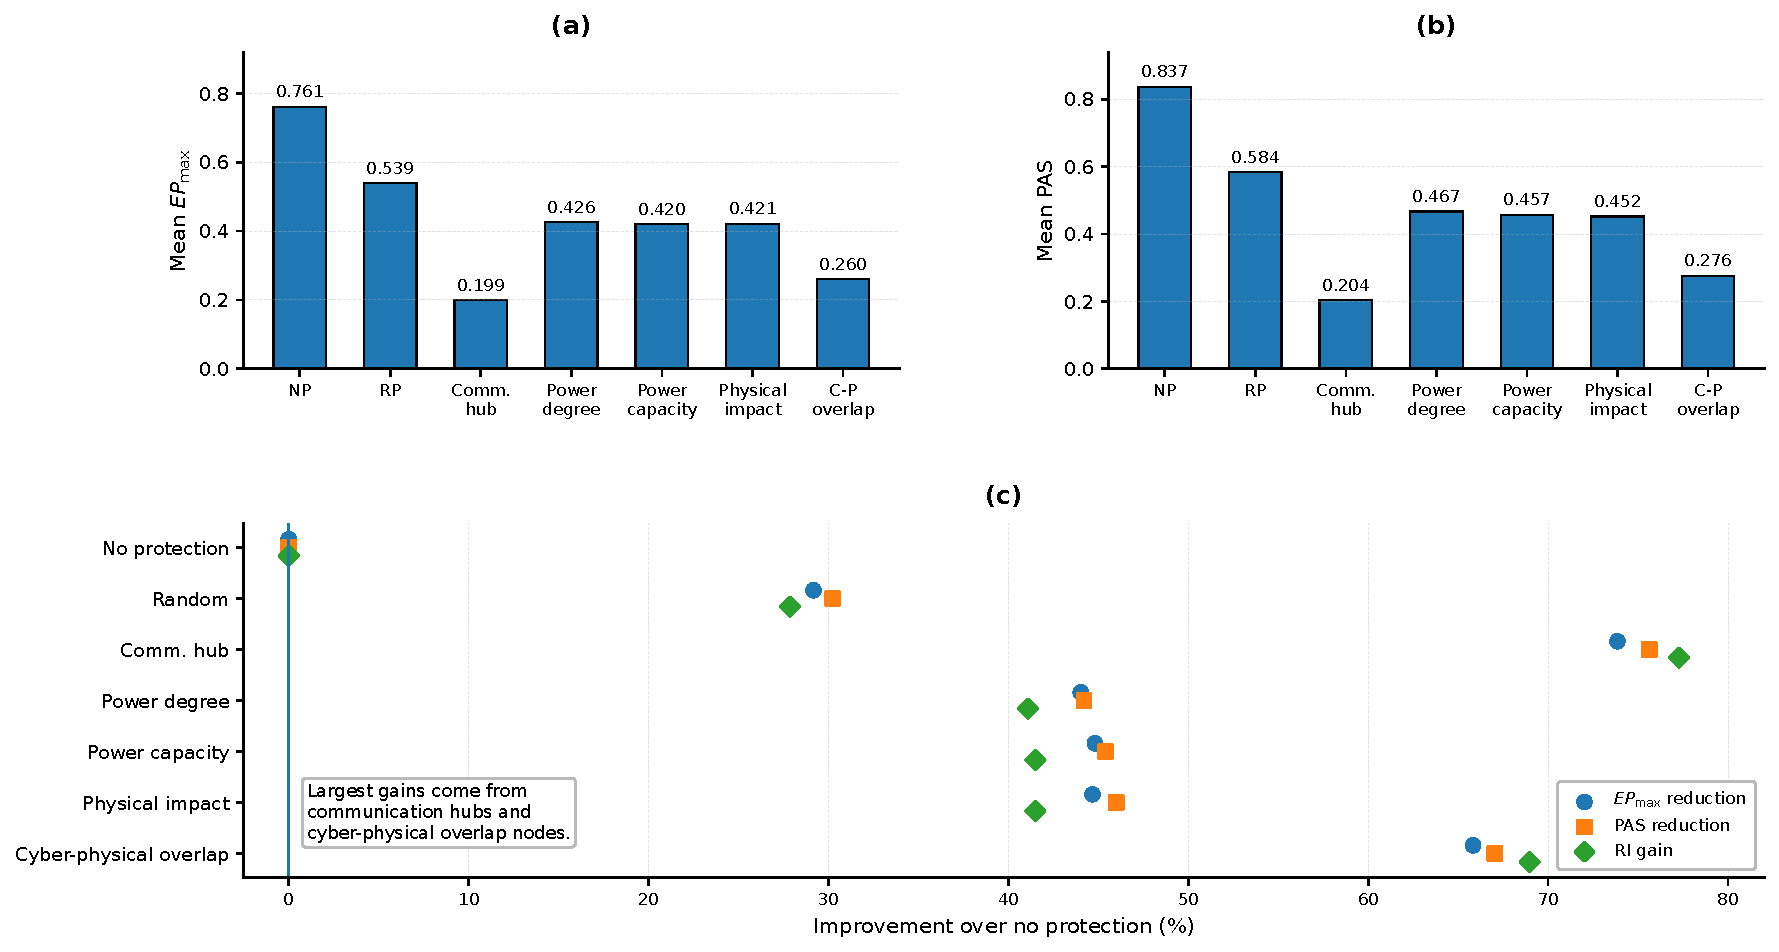
\includegraphics[width=0.98\textwidth]{figures/Figure3_revised_key_node_evidence_v1.pdf}
    \caption{Key-node protection performance under different protection priorities.}
    \label{fig:key_node_results}
\end{figure*}

The results show that communication hubs reduce the mean attacker payoff from $0.761$ under no protection to $0.199$, and reduce the mean PAS from $0.837$ to $0.204$. Meanwhile, the resilience index increases from $0.506$ to $0.897$. Cyber-physical overlap nodes also provide strong protection, reducing the mean attacker payoff to $0.260$ and increasing the resilience index to $0.855$. By contrast, power-degree, power-capacity, and physical-impact protection provide moderate but still meaningful improvements.

These findings reveal that cyber-layer containment is a dominant factor in this malware-induced CPPS setting. Since the attack originates from the communication layer, protecting communication hubs can suppress the spread before it crosses the cyber-physical interface. However, purely cyber-topological protection may not always be sufficient under heterogeneous coupling patterns. Cyber-physical overlap protection provides a complementary engineering principle by selecting nodes that are important to both malware diffusion and physical consequence. This motivates the policy-library design of DRAD-CF-MPC: the controller should be able to compare cyber-topological, physical-consequence, hybrid, and dynamic-risk policies under the same observed state instead of committing to a single definition of key node.

Fig.~\ref{fig:policy_switching} presents the adaptive policy-switching behavior and Safe-Guard mechanism of DRAD-CF-MPC. The policy selection distribution shows that CDP is selected most frequently, accounting for 46 out of the 90 coupling--information--budget scenarios, each evaluated at its worst attack timing. Rank-ensemble policies are selected in 20 scenarios, NP in 15 scenarios, CDP-PHYSICS in 6 scenarios, and CDP-PDP in 3 scenarios. This distribution indicates that DRAD-CF-MPC does not always replace the strong CDP baseline. Instead, it often retains CDP when it is predicted to be effective, while switching to other candidate policies under specific cyber-physical conditions.

\begin{figure*}[!tbp]
    \centering
    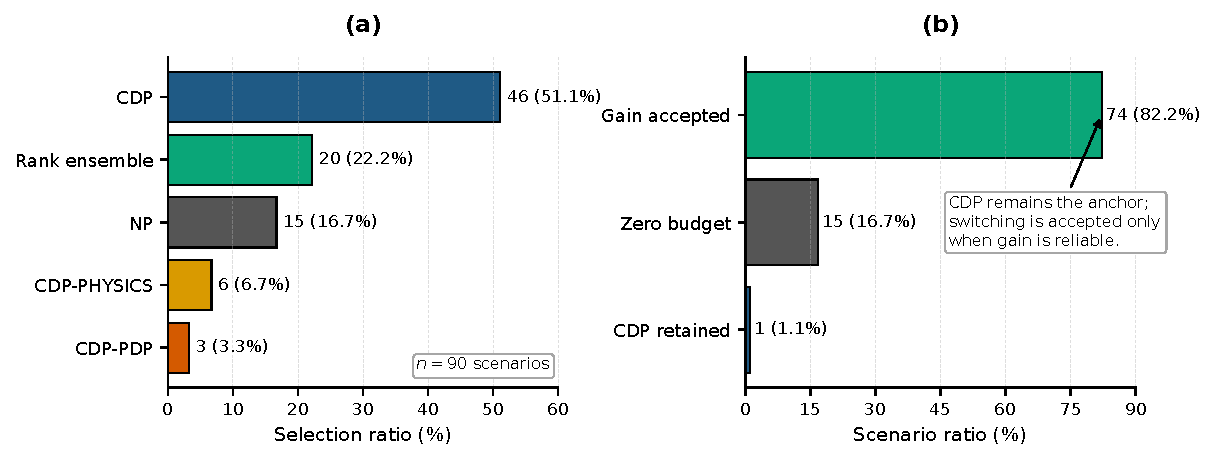
\includegraphics[width=0.98\textwidth]{figures/Figure4_revised_safeguarded_switching_v4_1780901110.pdf}
    \caption{Policy-selection and Safe-Guard outcomes of DRAD-CF-MPC.}
    \label{fig:policy_switching}
\end{figure*}

The Safe-Guard summary further confirms the conservative nature of the proposed controller. In 74 out of 90 scenarios, the Safe-Guard condition accepts the counterfactual best policy because the rollout predicts a reliable gain; in 45 of these accepted cases the best candidate coincides with CDP itself, so no actual policy change occurs. In 15 scenarios, zero-budget conditions prevent meaningful switching. In the remaining scenario, the Safe-Guard test rejects the candidate policy and falls back to CDP. Therefore, the Safe-Guard mechanism does not suppress adaptivity; rather, it ensures that adaptive switching is used only when the expected cyber-physical gain is sufficient.

The selected-policy distribution and budget analysis jointly support the second innovation. Multi-strategy selection is necessary because the best node-ranking principle changes across coupling, budget, and attack-information conditions. Safe-Guarding is also necessary because CDP is already a strong, interpretable policy; switching should occur only when counterfactual evidence indicates a reliable improvement. DRAD-CF-MPC therefore uses adaptivity as a controlled mechanism rather than as unconstrained policy chasing.

\subsection{Ablation of Counterfactual and Safe-Guard Components}
\label{subsec:incremental_results}

Table~\ref{tab:incremental_contribution} summarizes the incremental contribution of the proposed control architecture. Compared with no protection, random protection provides only limited improvement, whereas CDP substantially reduces the attacker payoff because communication hubs dominate malware diffusion. However, the full DRAD-CF-MPC architecture achieves the lowest mean $\mathrm{EP}_{\max}$ among all variants.

The comparison also shows that the proposed method is not merely a static risk-ranking rule. The largest component-level degradation occurs when MPC-based counterfactual evaluation is removed: the mean $\mathrm{EP}_{\max}$ increases from 0.289 to 0.341. Removing physical-consequence awareness or Safe-Guard fallback also weakens the final performance. These results support the design rationale that closed-loop counterfactual evaluation, cyber--physical consequence modeling, and conservative Safe-Guarded switching jointly contribute to the robustness improvement.

\begin{table}[!tbp]
\centering
\caption{Incremental contribution of DRAD-CF-MPC components.}
\label{tab:incremental_contribution}
\small
\begin{tabular}{lcc}
\toprule
\rowcolor{TableHeader}
Variant & Mean $EP_{\max}\downarrow$ & Gain vs. NP \\
\midrule
\rowcolor{RowWeak}
NP & 0.786 & 0.0\% \\
\rowcolor{RowNeutral}
RP & 0.567 & 27.9\% \\
\rowcolor{RowBaseline}
CDP & 0.298 & 62.1\% \\
\rowcolor{RowRisk}
DRAD-score & 0.348 & 55.7\% \\
\rowcolor{RowWeak}
w/o MPC & 0.341 & 56.6\% \\
\rowcolor{RowPhysical}
w/o physical consequence & 0.318 & 59.5\% \\
\rowcolor{RowScenario}
w/o Safe-Guard & 0.307 & 61.0\% \\
\rowcolor{RowProposed}
Full DRAD-CF-MPC & \best{0.289} & \best{63.2\%} \\
\bottomrule
\end{tabular}
\end{table}

The ablation results answer the third evaluation question. Counterfactual MPC provides the main mechanism for state-dependent policy choice, physical-consequence modeling connects cyber diffusion to affected service, and Safe-Guarding prevents unreliable departures from CDP. The full architecture is therefore a coupled design rather than an accumulation of independent heuristics.

\subsection{Degradation--Recovery Dynamics and Sensitivity Analysis}
\label{subsec:dynamic_evolution_results}

Fig.~\ref{fig:dynamic_evolution} provides a process-level explanation of how a malware attack evolves into physical degradation and restoration burden. This analysis directly connects internal CPPS state variables to the final evaluation metrics. The results show that, under no protection, malware rapidly accumulates in the communication layer, causing the number of active infectious nodes and affected physical buses to increase over time. Through the cyber-physical coupling matrix, infected communication nodes are mapped to physical buses, which in turn increases PAS in the power layer.

\begin{figure*}[!tbp]
    \centering
    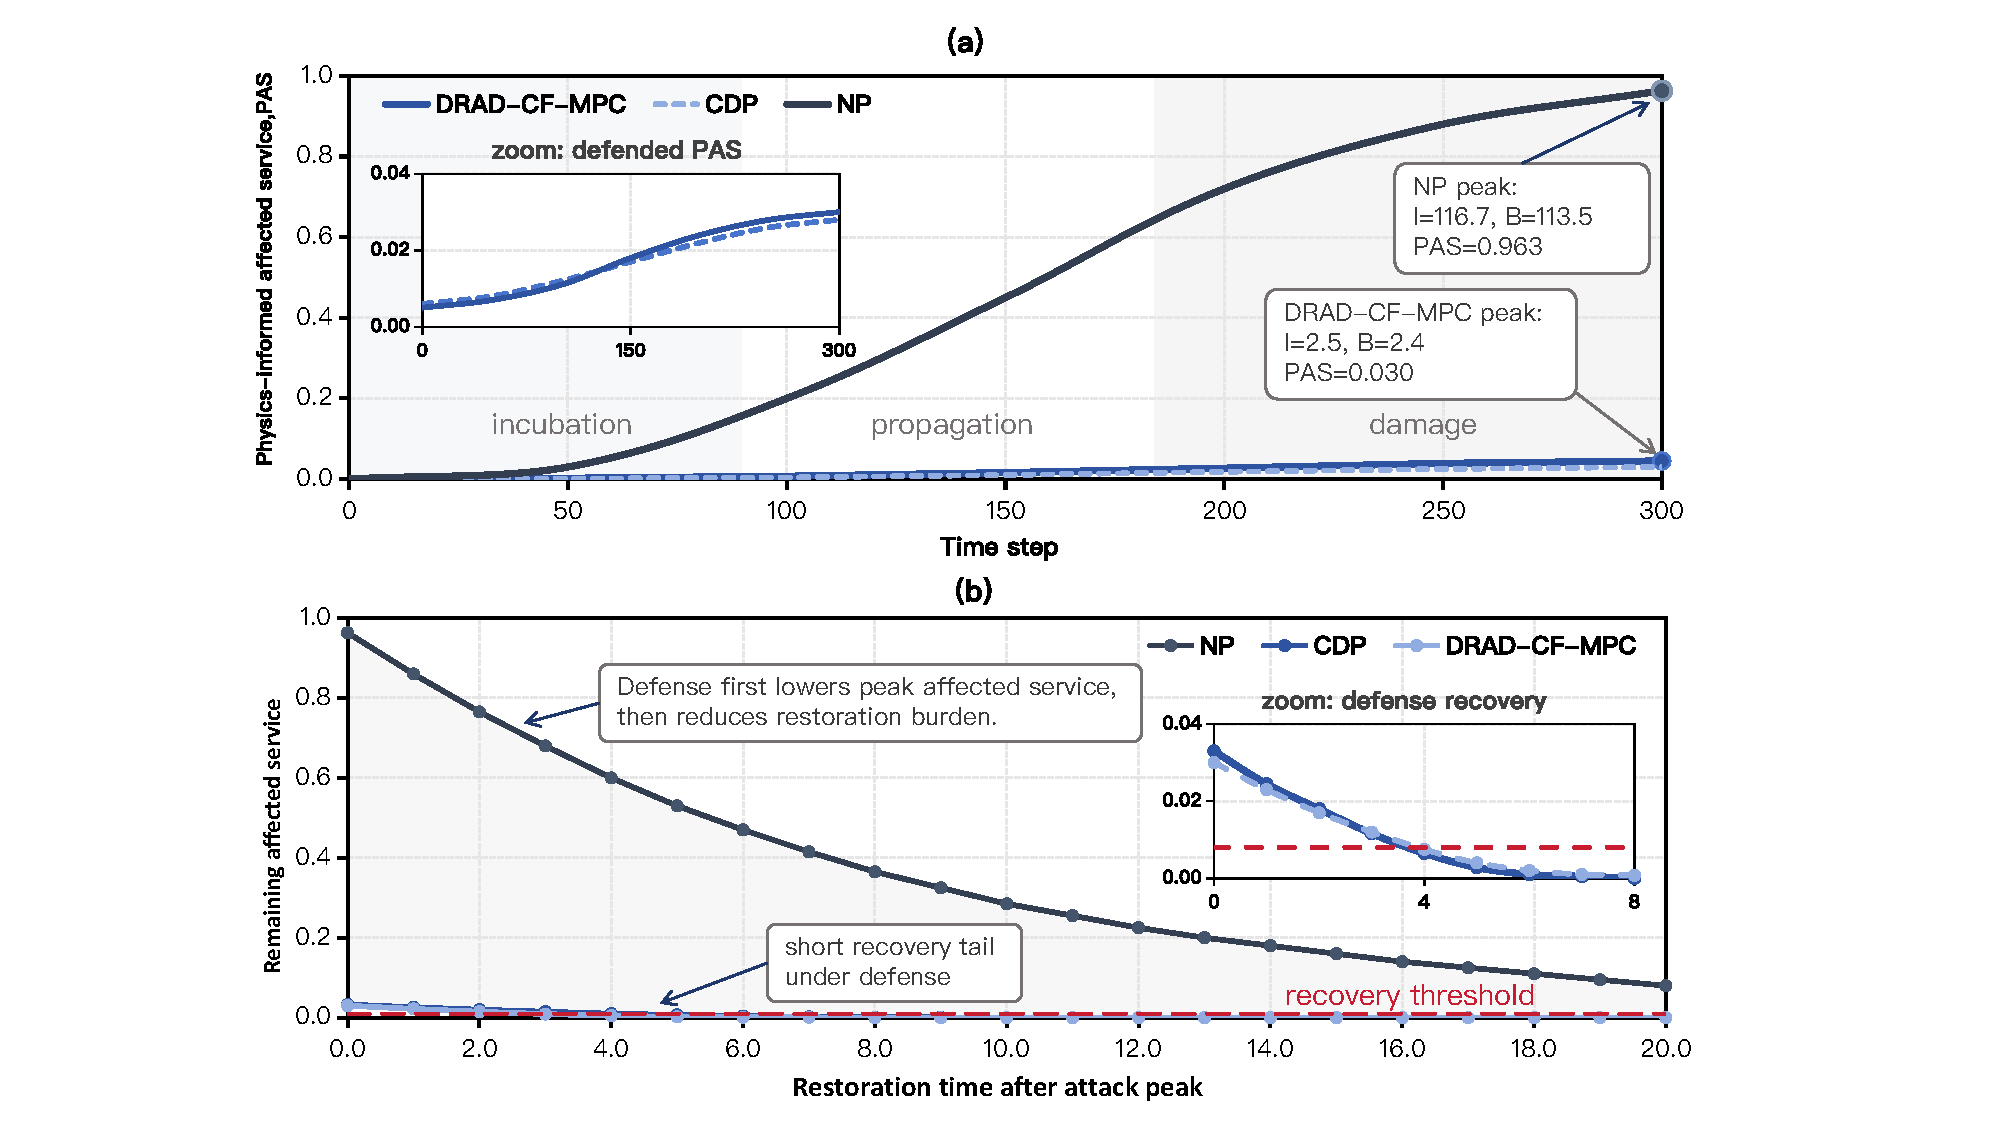
\includegraphics[width=0.98\textwidth]{figures/Figure5_process_evidence_clean.pdf}
    \caption{Dynamic degradation--recovery process under malware-induced cyber--physical attacks.}
    \label{fig:dynamic_evolution}
\end{figure*}

In the degradation trajectory of Fig.~\ref{fig:dynamic_evolution}(a), the no-protection case produces a rapid increase in PAS and reaches a severe peak, whereas CDP and DRAD-CF-MPC keep the affected-service trajectory close to the low-damage region. The annotated peak values further show that DRAD-CF-MPC substantially reduces peak infection, affected buses, and PAS compared with the unprotected case.

The recovery trajectory further shows that lowering the peak affected-service ratio also reduces the subsequent restoration burden. Under no protection, the remaining affected service decays slowly and stays above the recovery threshold for a much longer period. In contrast, DRAD-CF-MPC starts from a much smaller post-attack affected-service ratio and reaches the recovery threshold faster. The metric summary confirms that the proposed method improves both damage-oriented indicators and recovery-oriented indicators, including peak infection, affected buses, peak PAS, RT, RI, and RE.

Fig.~\ref{fig:sensitivity_results} reports the sensitivity of CPPS robustness to physically meaningful cyber-defense parameters. In addition to component ablation, this experiment varies the malware infection rate and detection capability, which directly control malware propagation stress and early containment ability.

\begin{figure*}[!tbp]
    \centering
    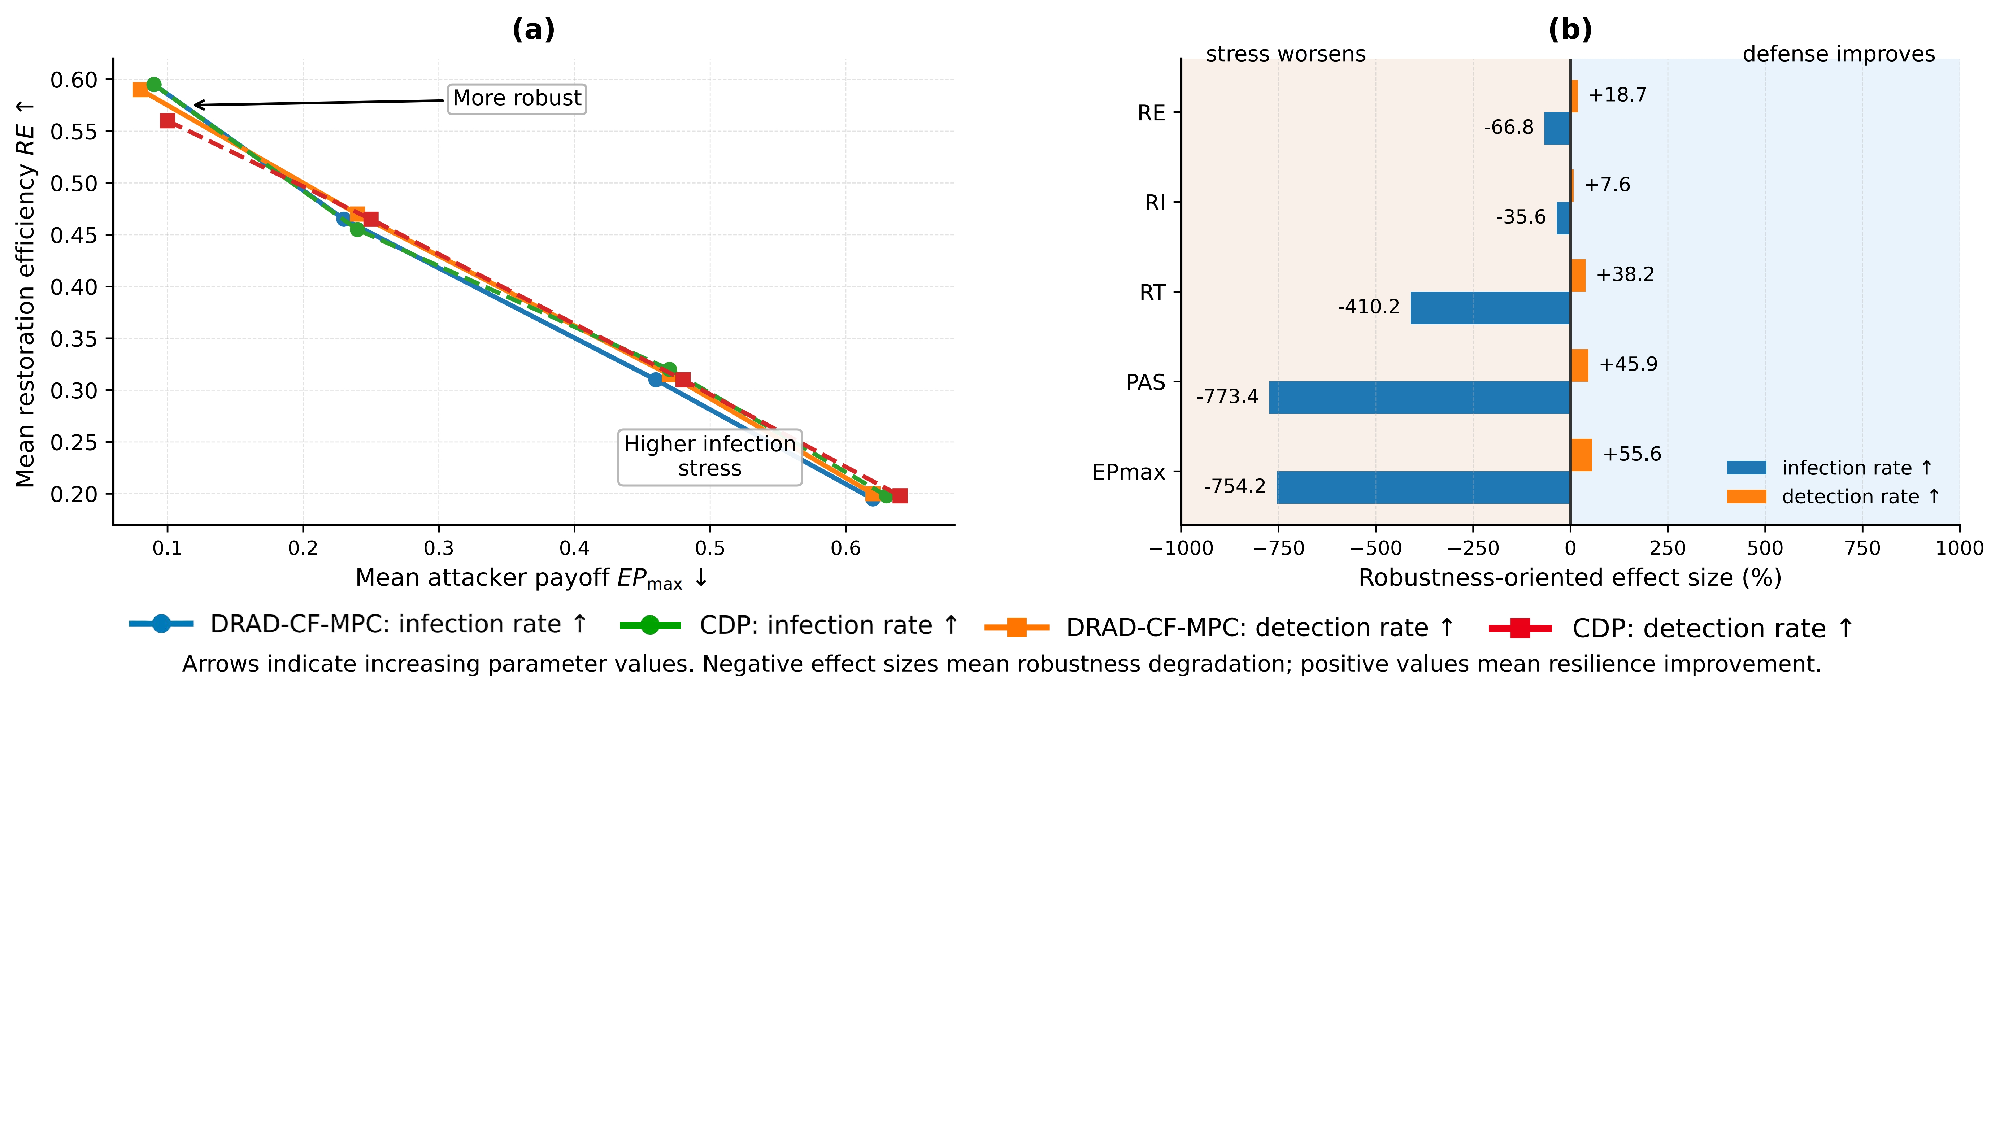
\includegraphics[width=0.98\textwidth]{figures/Figure6_sensitivity_two_panel_clean_v2.pdf}
    \caption{Sensitivity of CPPS robustness to infection and detection parameters.}
    \label{fig:sensitivity_results}
\end{figure*}

The robustness-state phase portrait shows that increasing the infection rate moves the CPPS toward higher attacker payoff and lower restoration efficiency. When the infection rate increases from $0.005$ to $0.03$, the system experiences a significant degradation in both attack suppression and recovery performance. This confirms that infection rate is a physical stress driver of malware-induced CPPS failure. In contrast, increasing detection capability improves early containment and shifts the system toward a more robust region. Detection enhancement is especially important for limiting the number of active infectious nodes before cyber compromise propagates into the physical layer.

The engineering effect-size analysis further quantifies the asymmetric influence of infection and detection parameters. Increasing infection rate has a strong negative effect on $\mathrm{EP}_{\max}$, PAS, RT, RI, and RE, whereas increasing detection rate has a positive but relatively smaller effect. This means that malware propagation intensity dominates CPPS robustness once the infection process becomes sufficiently aggressive. Nevertheless, improved detection remains beneficial because it reduces early propagation and helps preserve restoration efficiency.

The sensitivity results also indicate that the advantage of DRAD-CF-MPC should be interpreted as robust competitiveness rather than unconditional dominance at every parameter value. Under moderate detection and infection settings, DRAD-CF-MPC reduces EPmax relative to CDP. Under some high-detection or intermediate high-infection settings, CDP can be slightly better on selected metrics, reflecting the strength of communication-hub protection when malware containment dominates the damage process. Nevertheless, DRAD-CF-MPC maintains a comparable or better robustness profile across the tested parameter shifts and provides additional scenario-dependent improvement through Safe-Guarded counterfactual switching. This behavior is desirable for reliability-oriented defense because the adaptive controller avoids excessive deviation from a strong baseline while still exploiting beneficial switching opportunities.

\subsection*{Remark on Learning-Based Baselines}
DRAD-CF-MPC is designed as a sample-efficient, interpretable defense that requires no offline training and provides no-regret fallback to CDP via the Safe-Guard rule. A direct comparison with deep reinforcement learning (DRL) based defenses---such as DQN or PPO policies trained on the CPPS malware environment---is a natural extension. Such a comparison requires careful treatment of reward shaping, training stability under rare physical-activation events, and the interpretability trade-off that motivates the present work. This comparison is identified as a primary direction for future work.

\section{Conclusion}
\label{sec:conclusion}

This paper proposed DRAD-CF-MPC, a Safe-Guarded counterfactual defense framework for malware-resilient cyber--physical power systems. The framework reformulates malware defense as a closed-loop CPPS intervention problem, evaluates interpretable candidate policies through same-state counterfactual lookahead, and accepts adaptive switching only when the Safe-Guard condition indicates a reliable gain over a strong baseline. By linking malware diffusion, PAS, and post-attack restoration, the method evaluates both peak affected service and recovery burden. The simulation results show that conservative counterfactual adaptation can improve CPPS resilience without abandoning interpretable baseline protection rules. This supports the main design message of the paper: reliable CPPS malware defense should combine interpretable baseline protection with cautious counterfactual adaptation rather than pursue unconstrained switching.

\section*{Acknowledgment}
This research was supported by the National Natural Science Foundation of China under Grants No. 62403174 and 62573170.

\bibliographystyle{IEEEtran}
\bibliography{cas-refs}

\ifincludeauthorbios
\begin{IEEEbiography}[{\includegraphics[width=1in,height=1.25in,clip,keepaspectratio]{authors/cheng.jpg}}]{Weihao Cheng}
Biography text to be completed before the final IEEE production version.
\end{IEEEbiography}

\begin{IEEEbiography}[{\includegraphics[width=1in,height=1.25in,clip,keepaspectratio]{authors/tu.jpg}}]{Haicheng Tu}
Biography text to be completed before the final IEEE production version.
\end{IEEEbiography}

\begin{IEEEbiography}[{\includegraphics[width=1in,height=1.25in,clip,keepaspectratio]{authors/xia.jpg}}]{Yongxiang Xia}
Biography text to be completed before the final IEEE production version.
\end{IEEEbiography}

\begin{IEEEbiography}[{\includegraphics[width=1in,height=1.25in,clip,keepaspectratio]{authors/chen.jpg}}]{Xi Chen}
Biography text to be completed before the final IEEE production version.
\end{IEEEbiography}
\fi

\end{document}
